\documentclass{beamer}
\usepackage{amssymb}% http://ctan.org/pkg/amssymb
\usepackage{pifont}% http://ctan.org/pkg/pifont
\usepackage{subcaption}
\usepackage{comment}
\usepackage{csvsimple, booktabs}
\usepackage{pgffor}%
\usepackage{transparent}

\usepackage{ifpdf}%
  \ifpdf%
    \DeclareGraphicsExtensions{.pdf,.png,.jpg}%
  \else%
    \DeclareGraphicsExtensions{.eps,.ps}%
  \fi%
\logo{
\includegraphics[width=15mm,scale=0.2]{uib_01.png}}
\beamertemplatenavigationsymbolsempty
\usetheme{PaloAlto}
%\usecolortheme{wolverine}
%\setbeamertemplate{headline}{} % not showing on top
\setbeamertemplate{footline}[page number]


\newcommand*{\List}{%
../gen/det/1660309200.jpg,
../gen/det/1660302000.jpg,
../gen/det/1660294800.jpg,
../gen/det/1660320000.jpg,
../gen/det/1660287600.jpg,
../gen/det/1660298400.jpg,
../gen/det/1660305600.jpg,
../gen/det/1660316400.jpg,
../gen/det/1660291200.jpg
}%


\newcommand{\beamerfigure}[1]{%
  \begin{frame}%
        \begin{figure}
            \centering
            \includegraphics[width=\textwidth]{"#1"}
        \end{figure}
  \end{frame}%
}%

%Information to be included in the title page:
\title{Crowd counting using OpenCV and Python}
\author{Martí Gelabert Gómez}
\institute{University of the Balearic Islands}
\date{\today}

\AtBeginSection[]{
  \begin{frame}
  \vfill
  \centering
  \begin{beamercolorbox}[sep=8pt,center,shadow=true,rounded=true]{title}
    \usebeamerfont{title}\insertsectionhead\par%
  \end{beamercolorbox}
  \vfill
  \end{frame}
}

\begin{document}

\frame{\titlepage}

\section*{Introduction}
\begin{frame}

    \frametitle{Objective}
    We need to generate and algorithm capable of \textbf{crowd counting}...\medskip\pause
    
    So we need  to :
    \begin{itemize}
        
        \item<2-> Have some kind of ground truth
        \item<3-> An algorithm to Detect persons
        \item<4-> And be able to quantify our performance
    \end{itemize}

\end{frame}


\begin{frame}
    \frametitle{Labeling}
    First, we need to \textbf{label} our images and establish some kind of \textbf{criteria} to decide which persons to label. 
\end{frame}

\begin{frame}
    \frametitle{Occlusions}
\begin{figure}
    \centering
    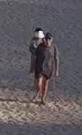
\includegraphics{lab/oclusion.png}
\end{figure}
\end{frame}

\begin{frame}
    \frametitle{Compact information}
\begin{figure}
    \centering
    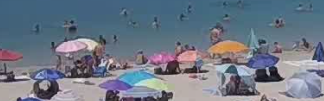
\includegraphics{lab/shore.png}
\end{figure}
\end{frame}

\begin{frame}
    \frametitle{Masked areas}

    \centering

    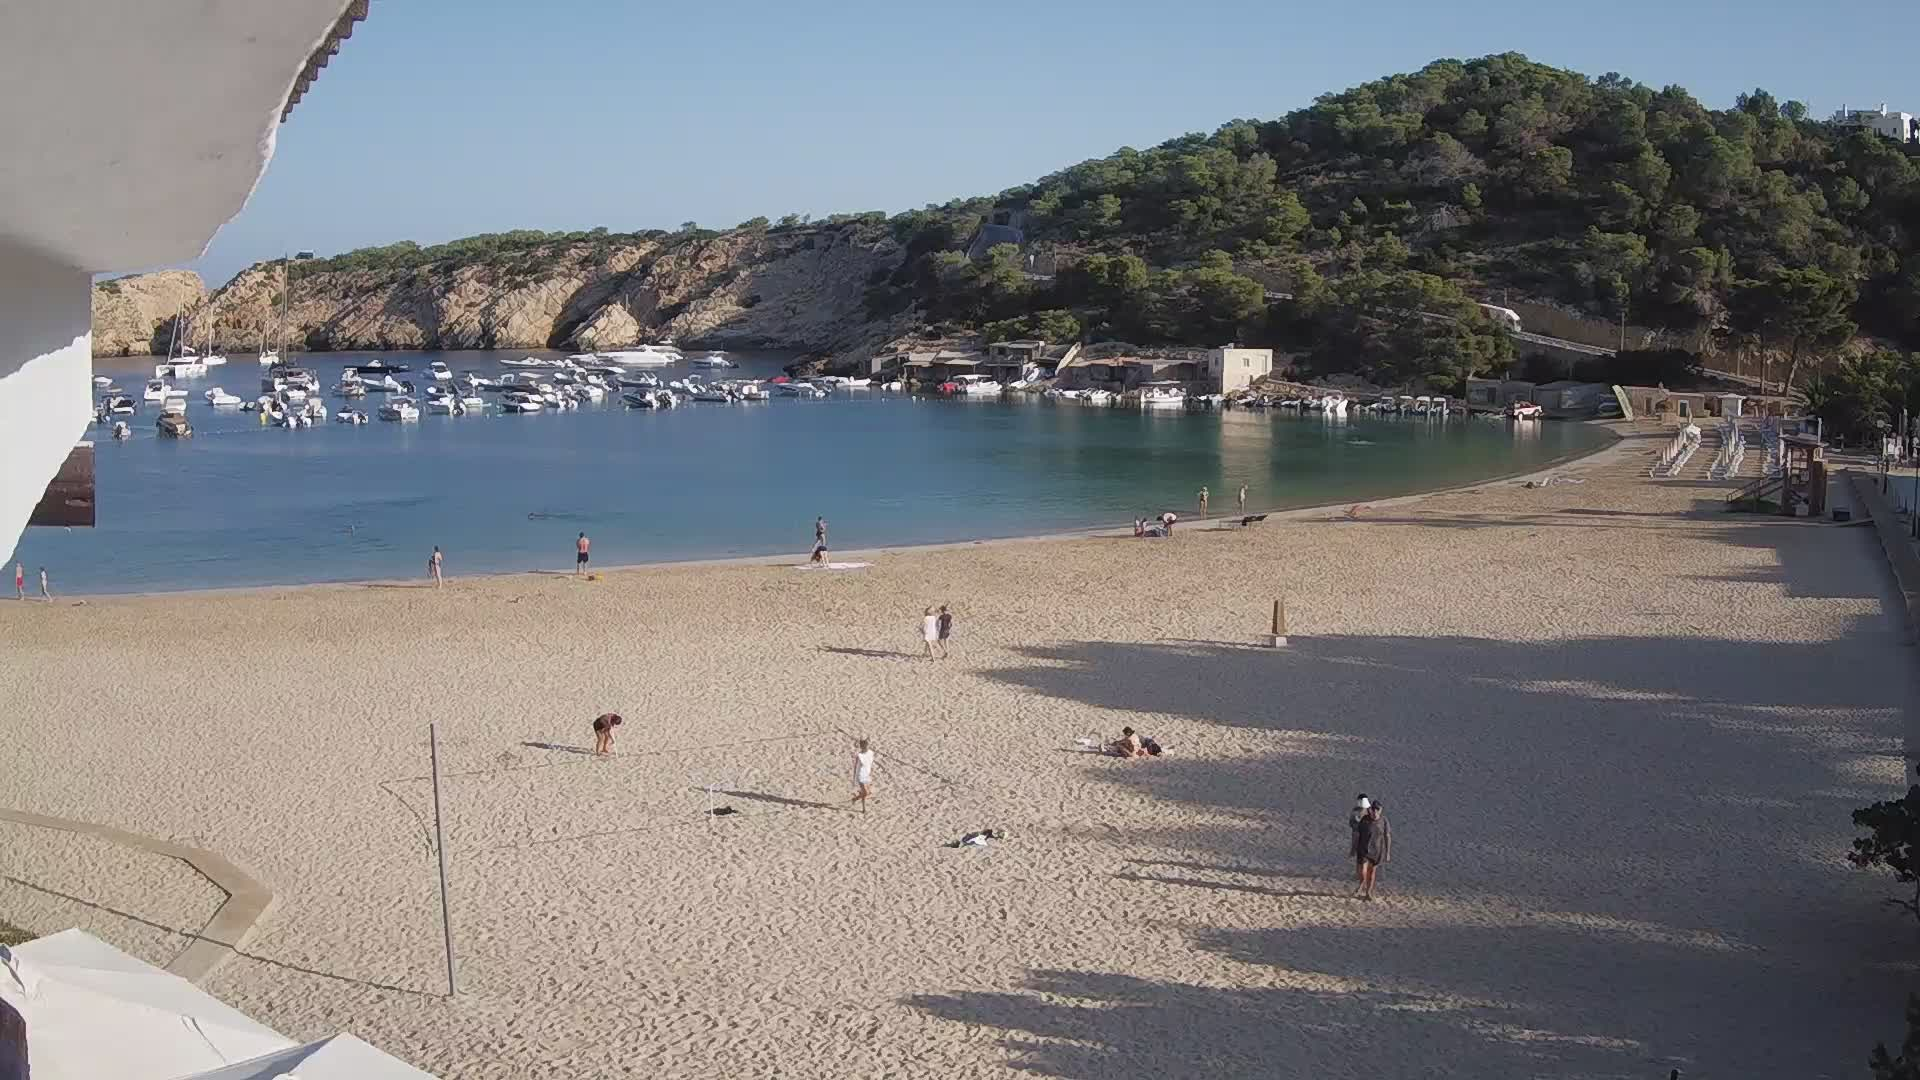
\includegraphics[width=\textwidth,]{../Gelabert/1660287600.jpg}
    \vspace*{-6.25cm}
   {\transparent{0.8} 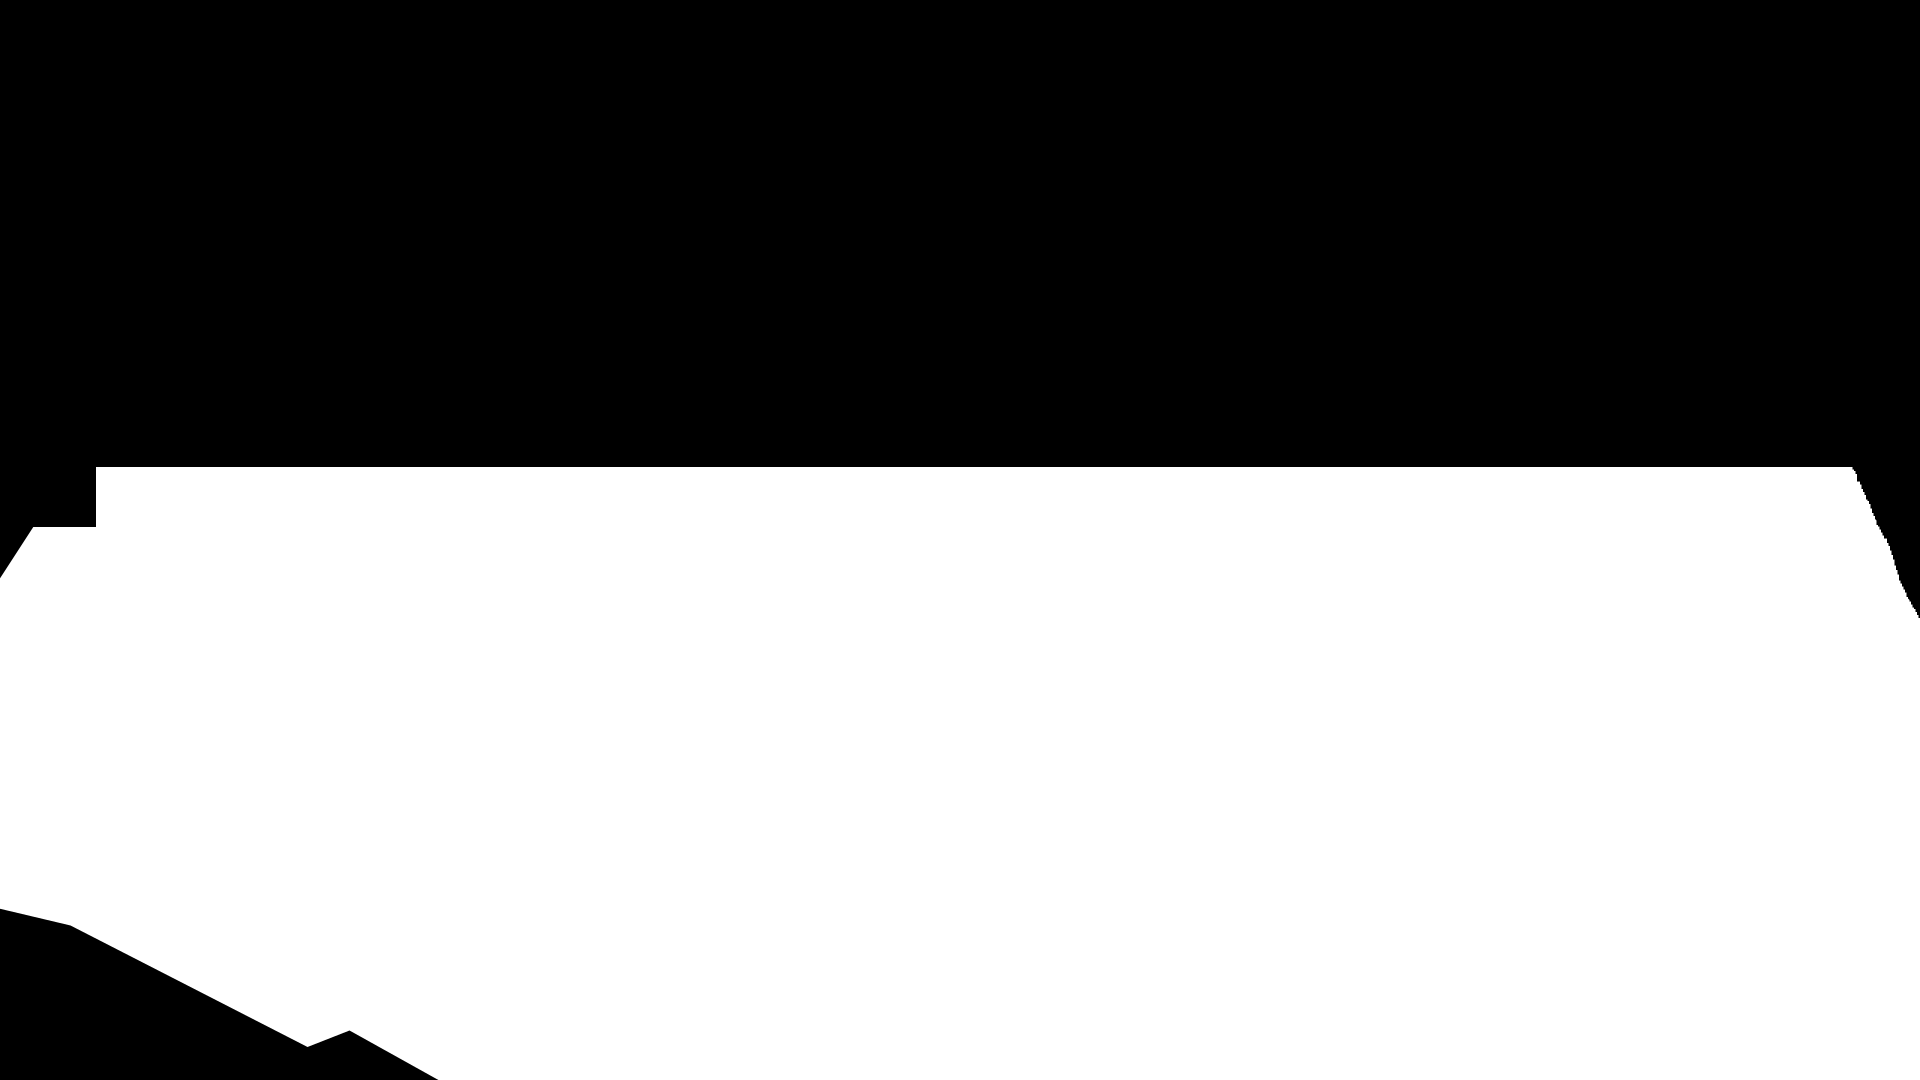
\includegraphics[width=\textwidth,]{../mask.png}}

\end{frame}

%%%%%%%%%%%%%%%%%%%%%%%%%%%%%%5


\begin{frame}
    \frametitle{Person detection}
    Now, we need a way for \textbf{detecting people}:
    \begin{itemize}
        \item<2-> Gabor filtering  \pause {\color{red} \ding{55}}
        \item<3-> Edge detector  \pause {\color{red} \ding{55}}
        \item<4-> Applying derivatives \pause {\color{red} \ding{55}}
        \item<5-> Background removal  {\color{green} \checkmark}
    \end{itemize}
     
\end{frame}

%\frame{\tableofcontents}

\section{Background Removal}
    \begin{frame}
        \frametitle{Background Removal}
        \begin{figure}
            \centering
            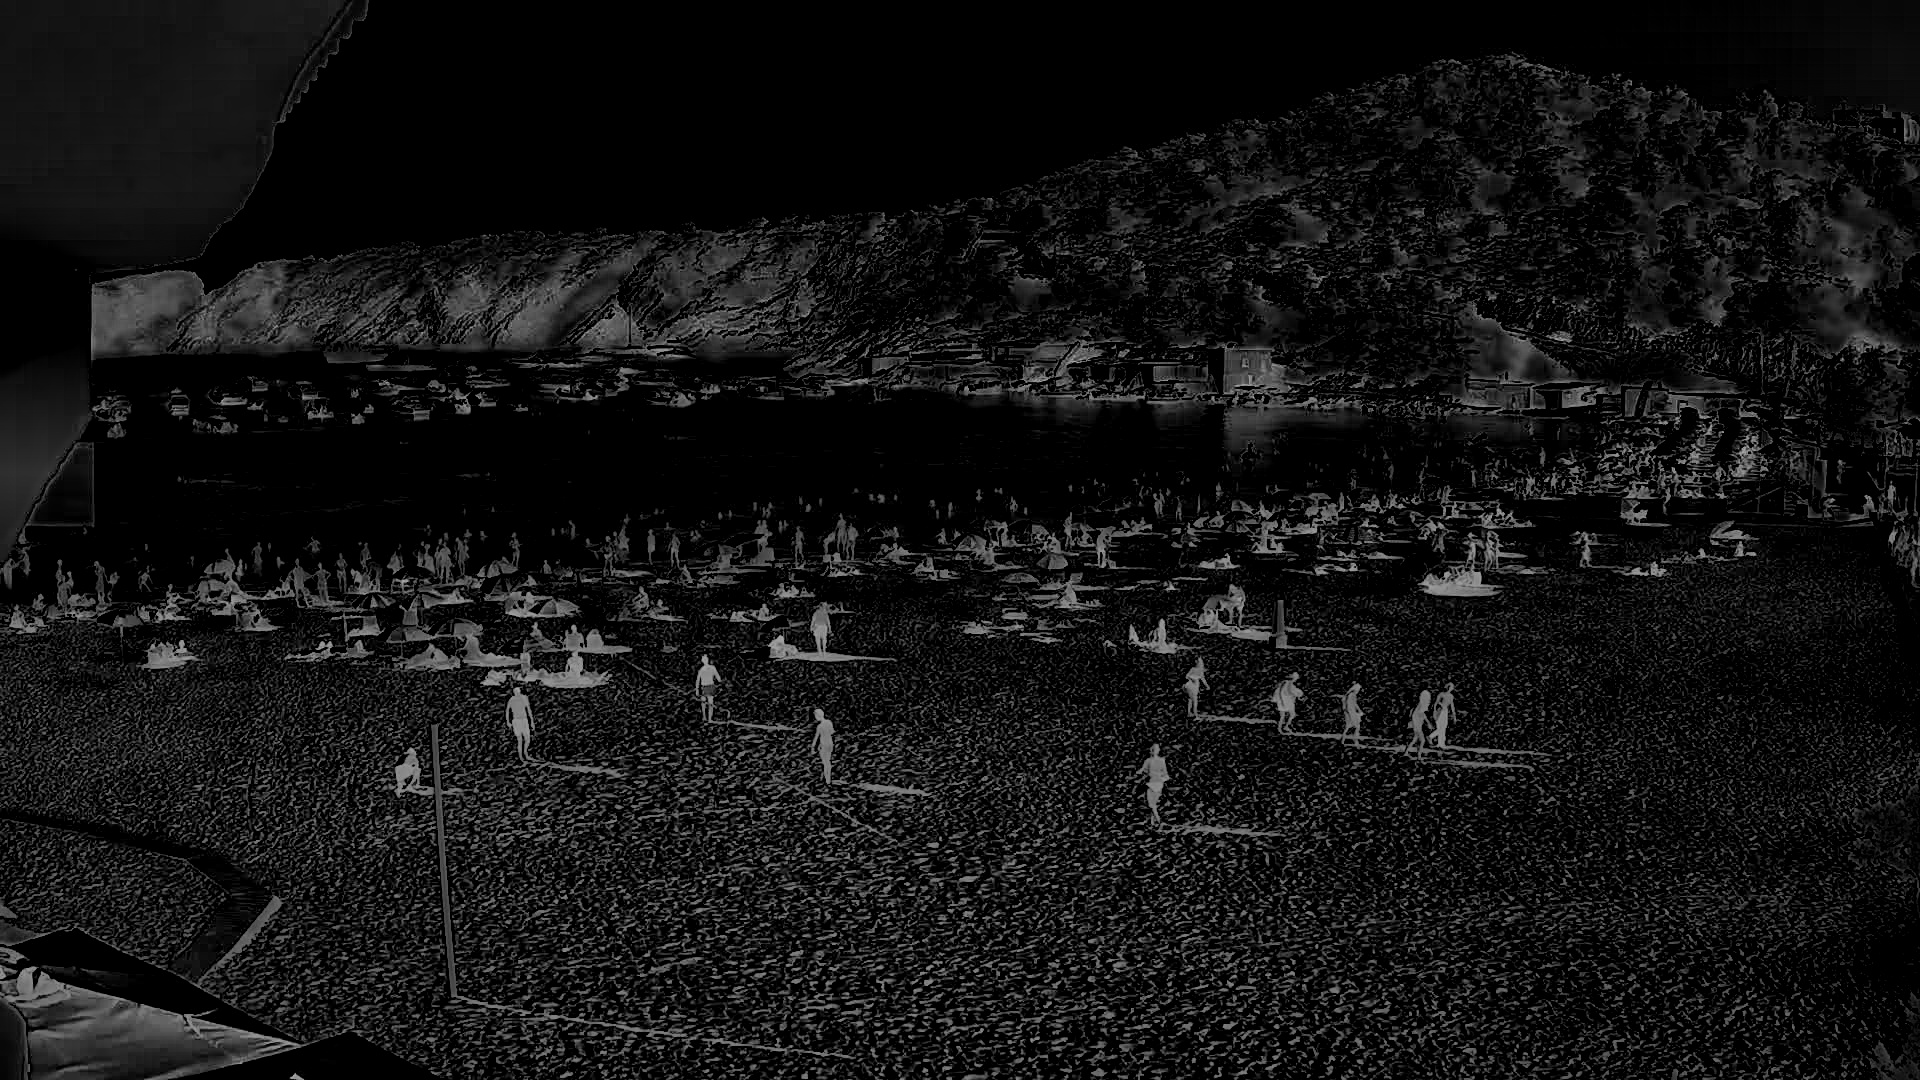
\includegraphics[width=\textwidth]{../gen/sub/1660320000.jpg}
        \end{figure}
    \end{frame}

\begin{frame}

    \begin{block}{Remark}
        The operations will be done using \textbf{grey scale} images.
        \end{block}\medskip
        
        We need to do something with the \textbf{illumination} of the images and improve the \textbf{contrast}.
        
\end{frame}
\subsection*{CLAHE}

\begin{comment}
    \begin{frame}
        \frametitle{CLAHE}
        We need to do something with the illumination of the images.
        \begin{columns}[c]
            % create the column with the first image, that occupies
            % half of the slide
                \begin{column}{.5\textwidth}
                \begin{figure}
                    \centering
                    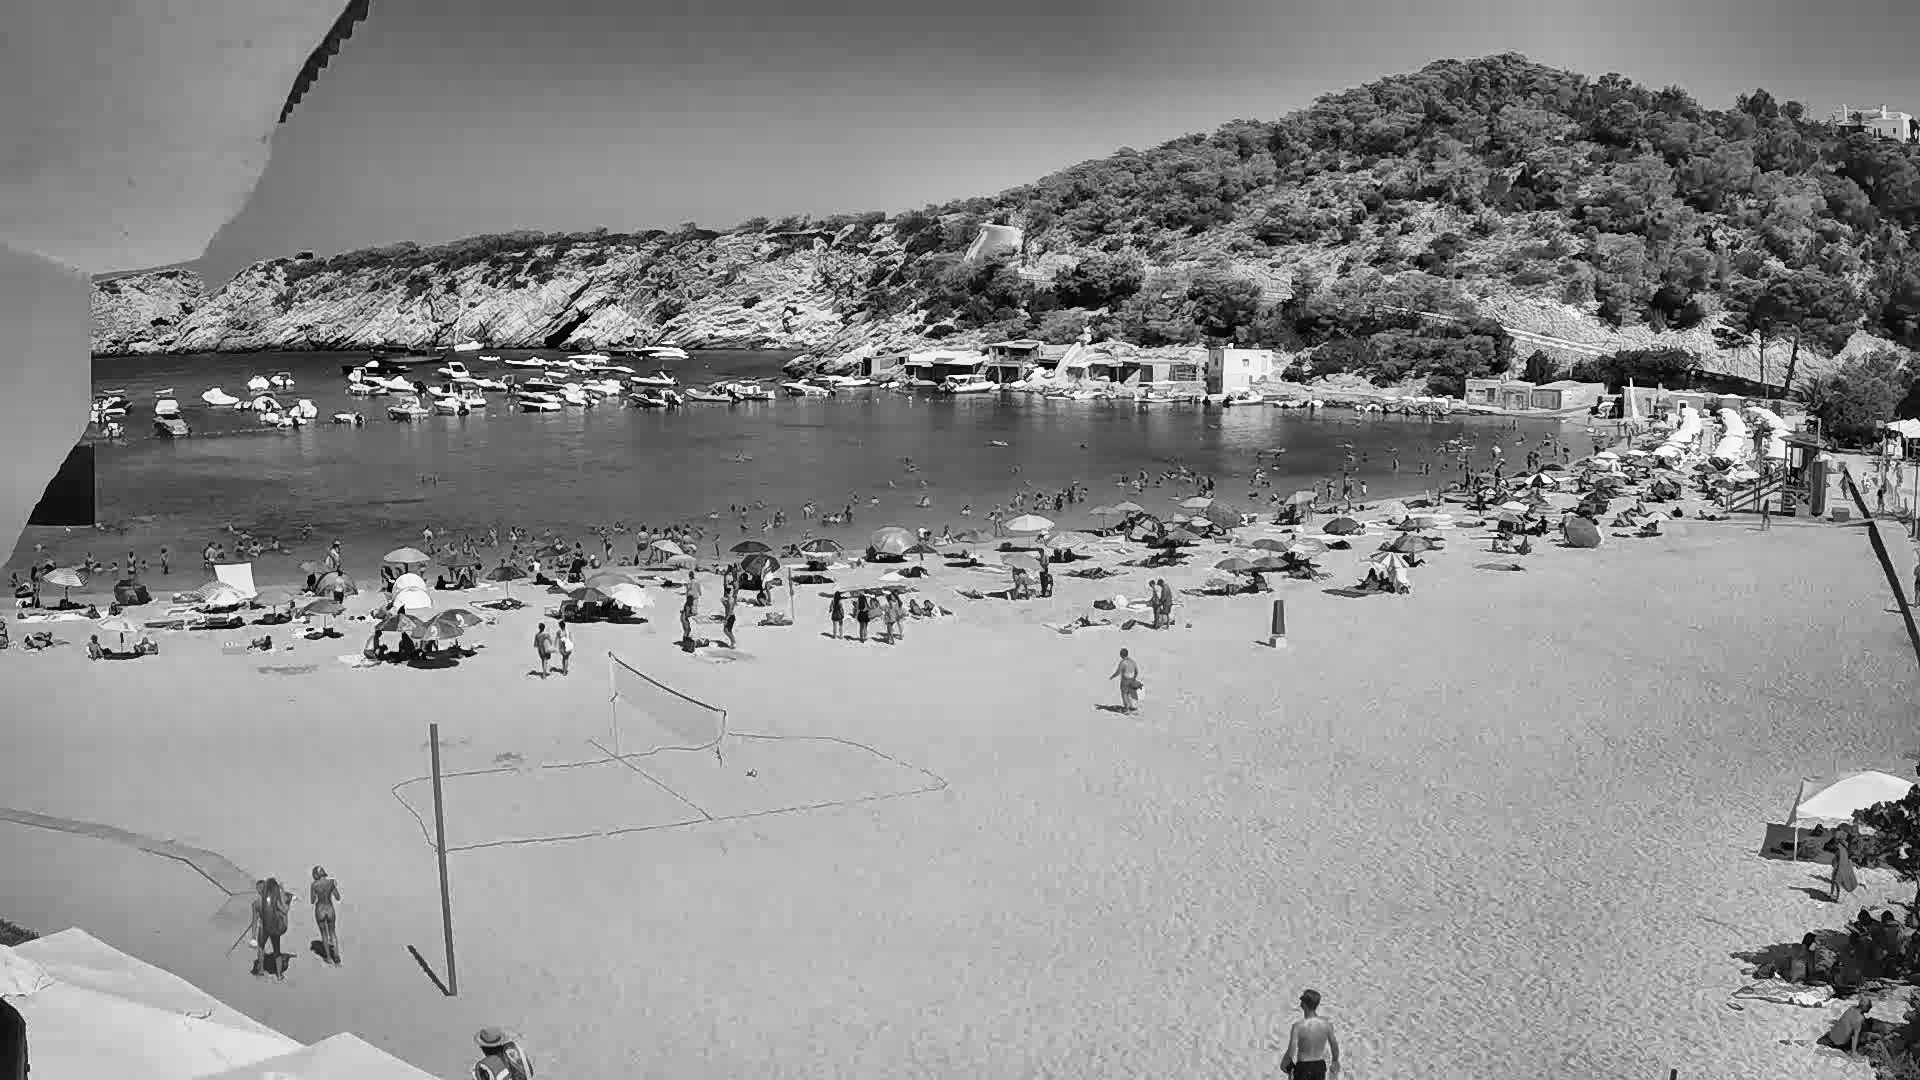
\includegraphics[width=\textwidth]{../gen/equ/1660298400.jpg}
                    
                \end{figure}      
                \end{column}
            % create the column with the second image, that also
            % occupies half of the slide
                \begin{column}{.5\textwidth}
                \begin{figure}
                    \centering
                    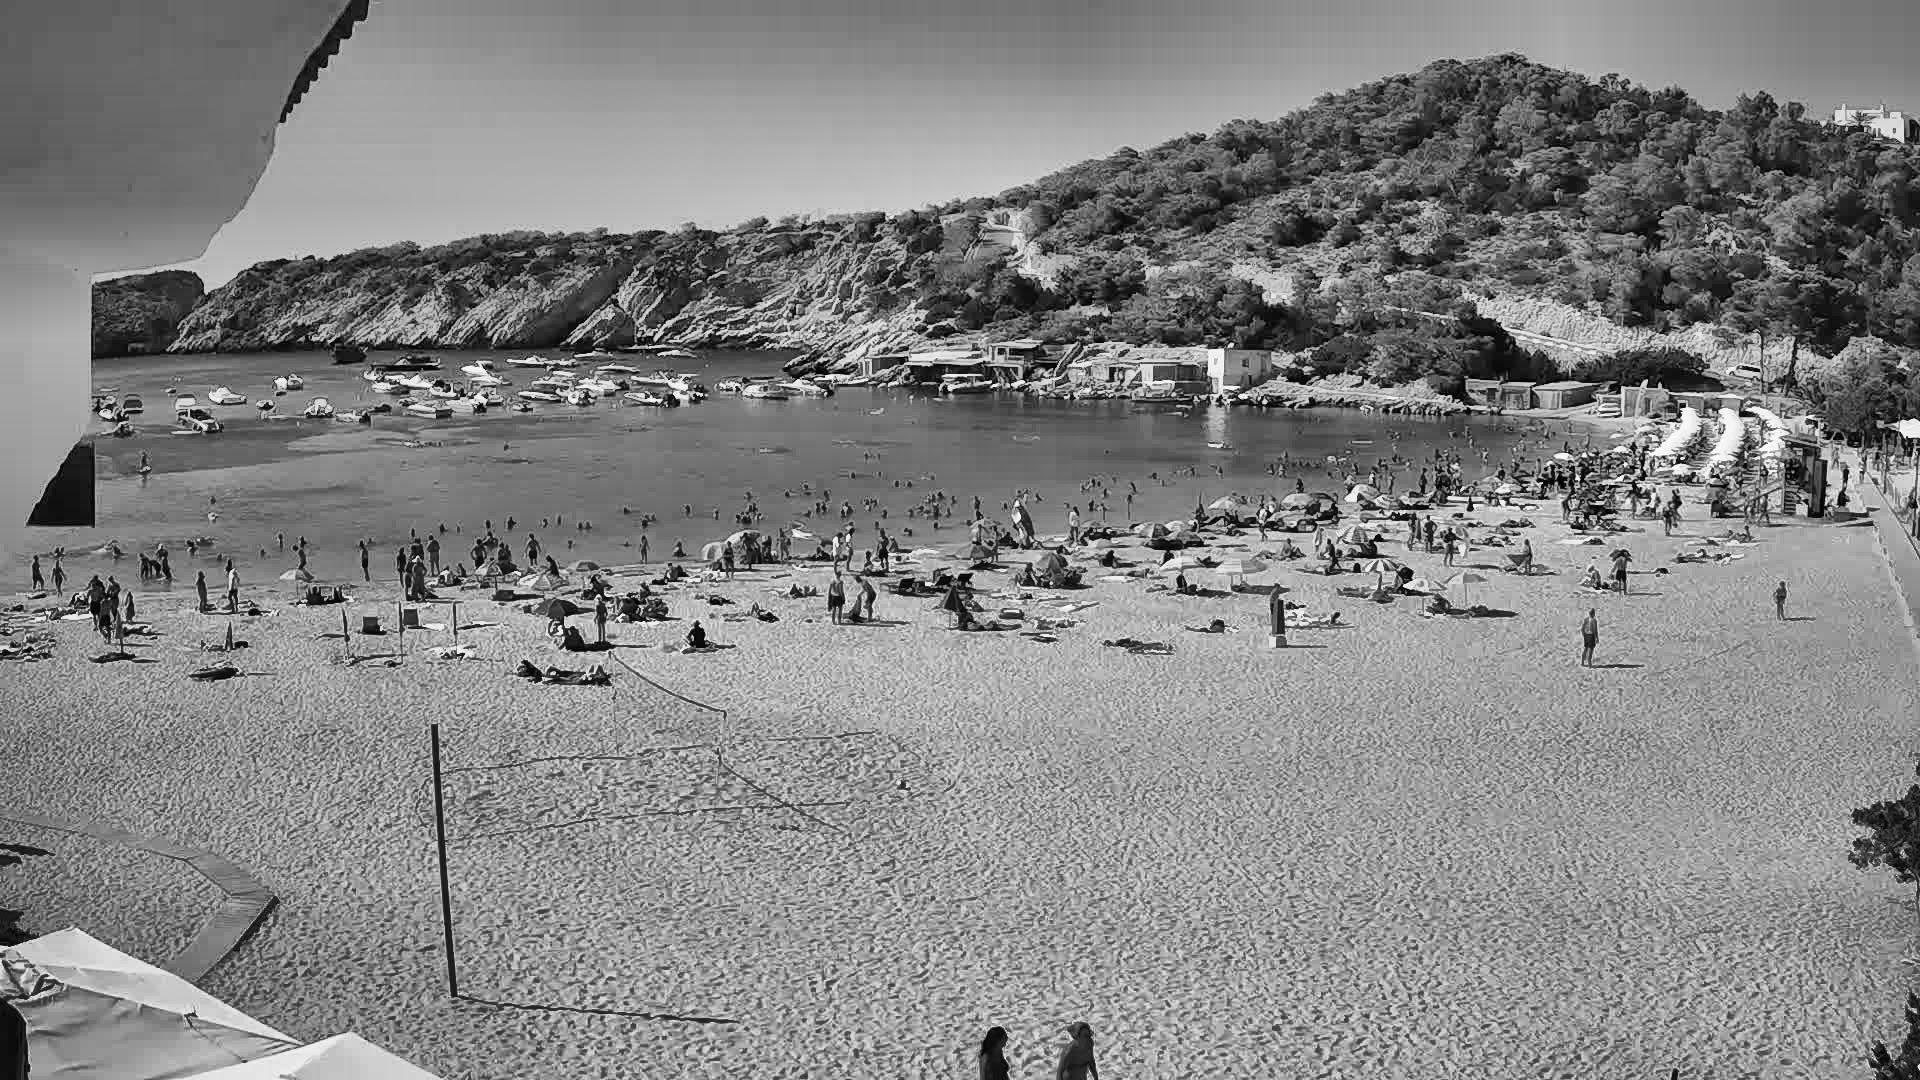
\includegraphics[width=\textwidth]{../gen/equ/1660316400.jpg}                 
                \end{figure}
                \end{column}
            \end{columns}
    \end{frame}
\end{comment}

\begin{frame}
    \frametitle{CLAHE}
    \centering
    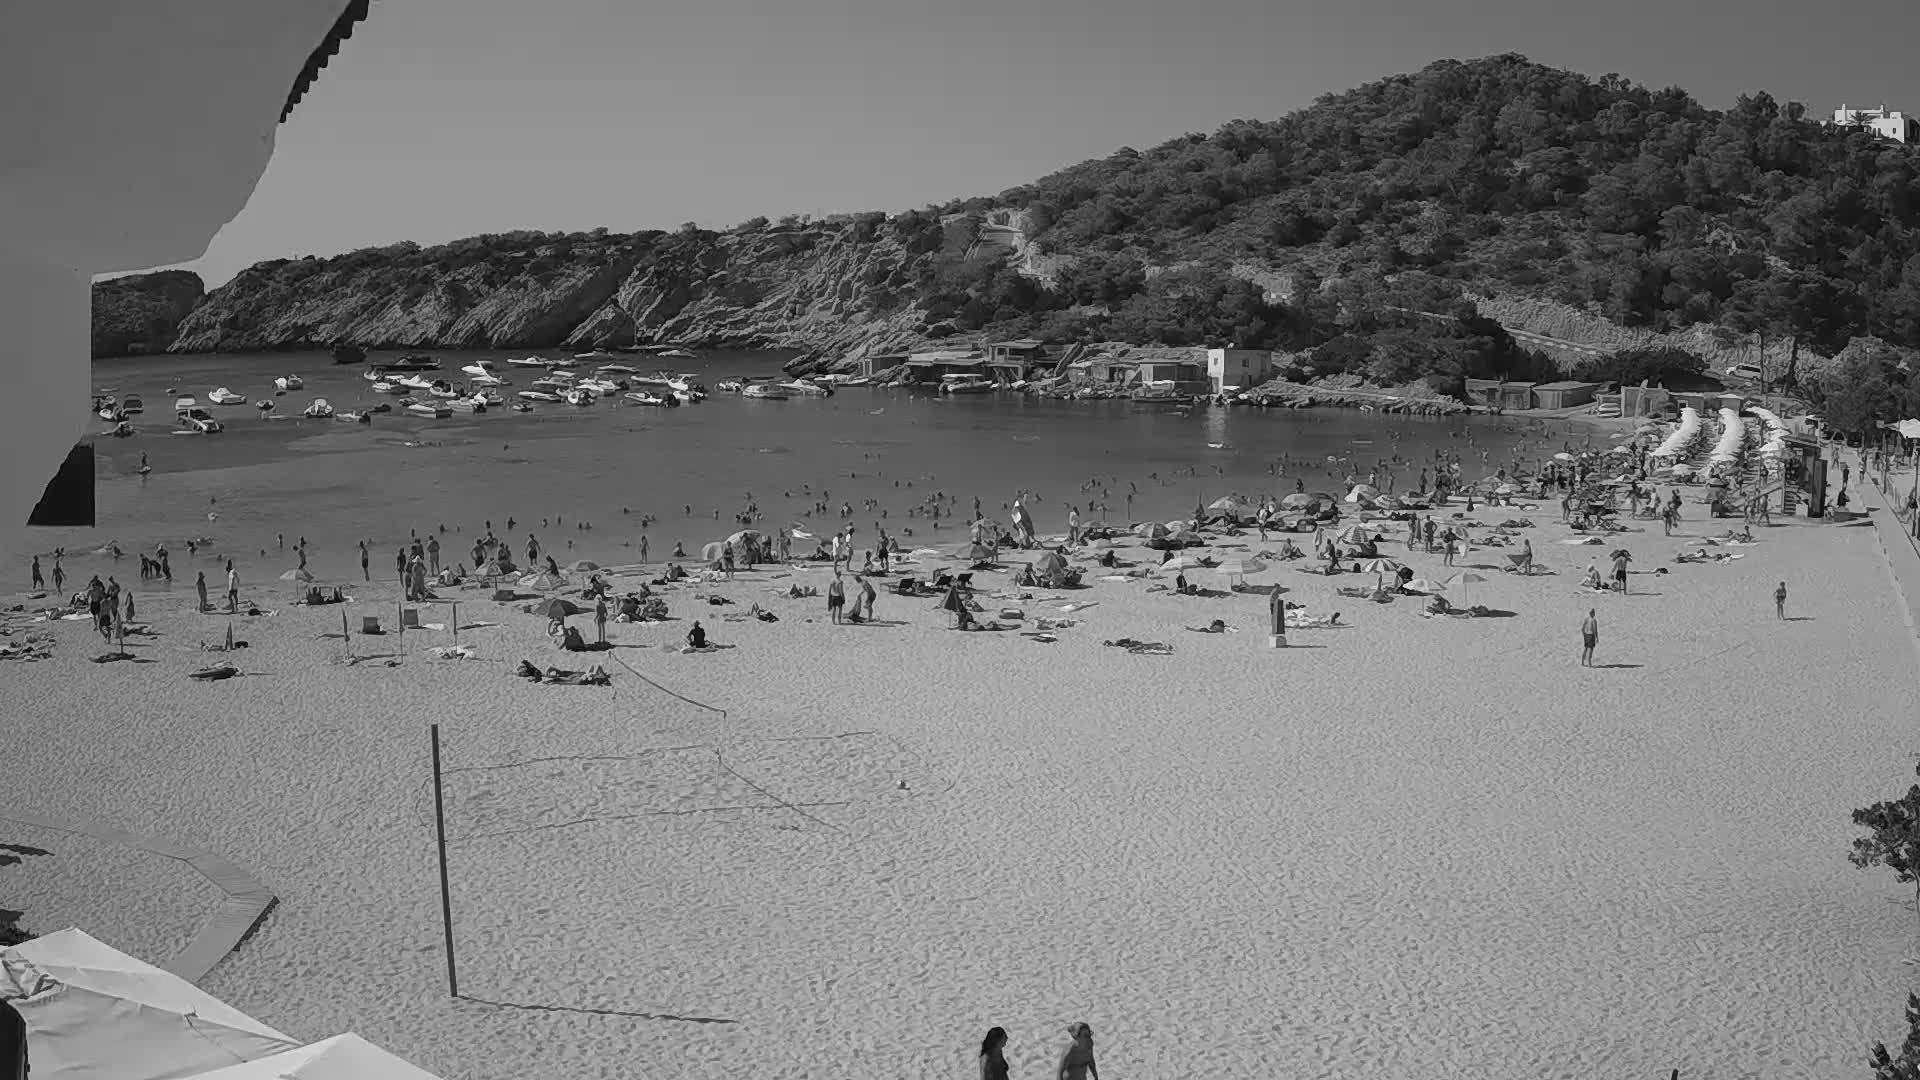
\includegraphics[width=\textwidth]{../gen/gray/1660316400.jpg}
  
\end{frame}

\begin{frame}
    \centering
    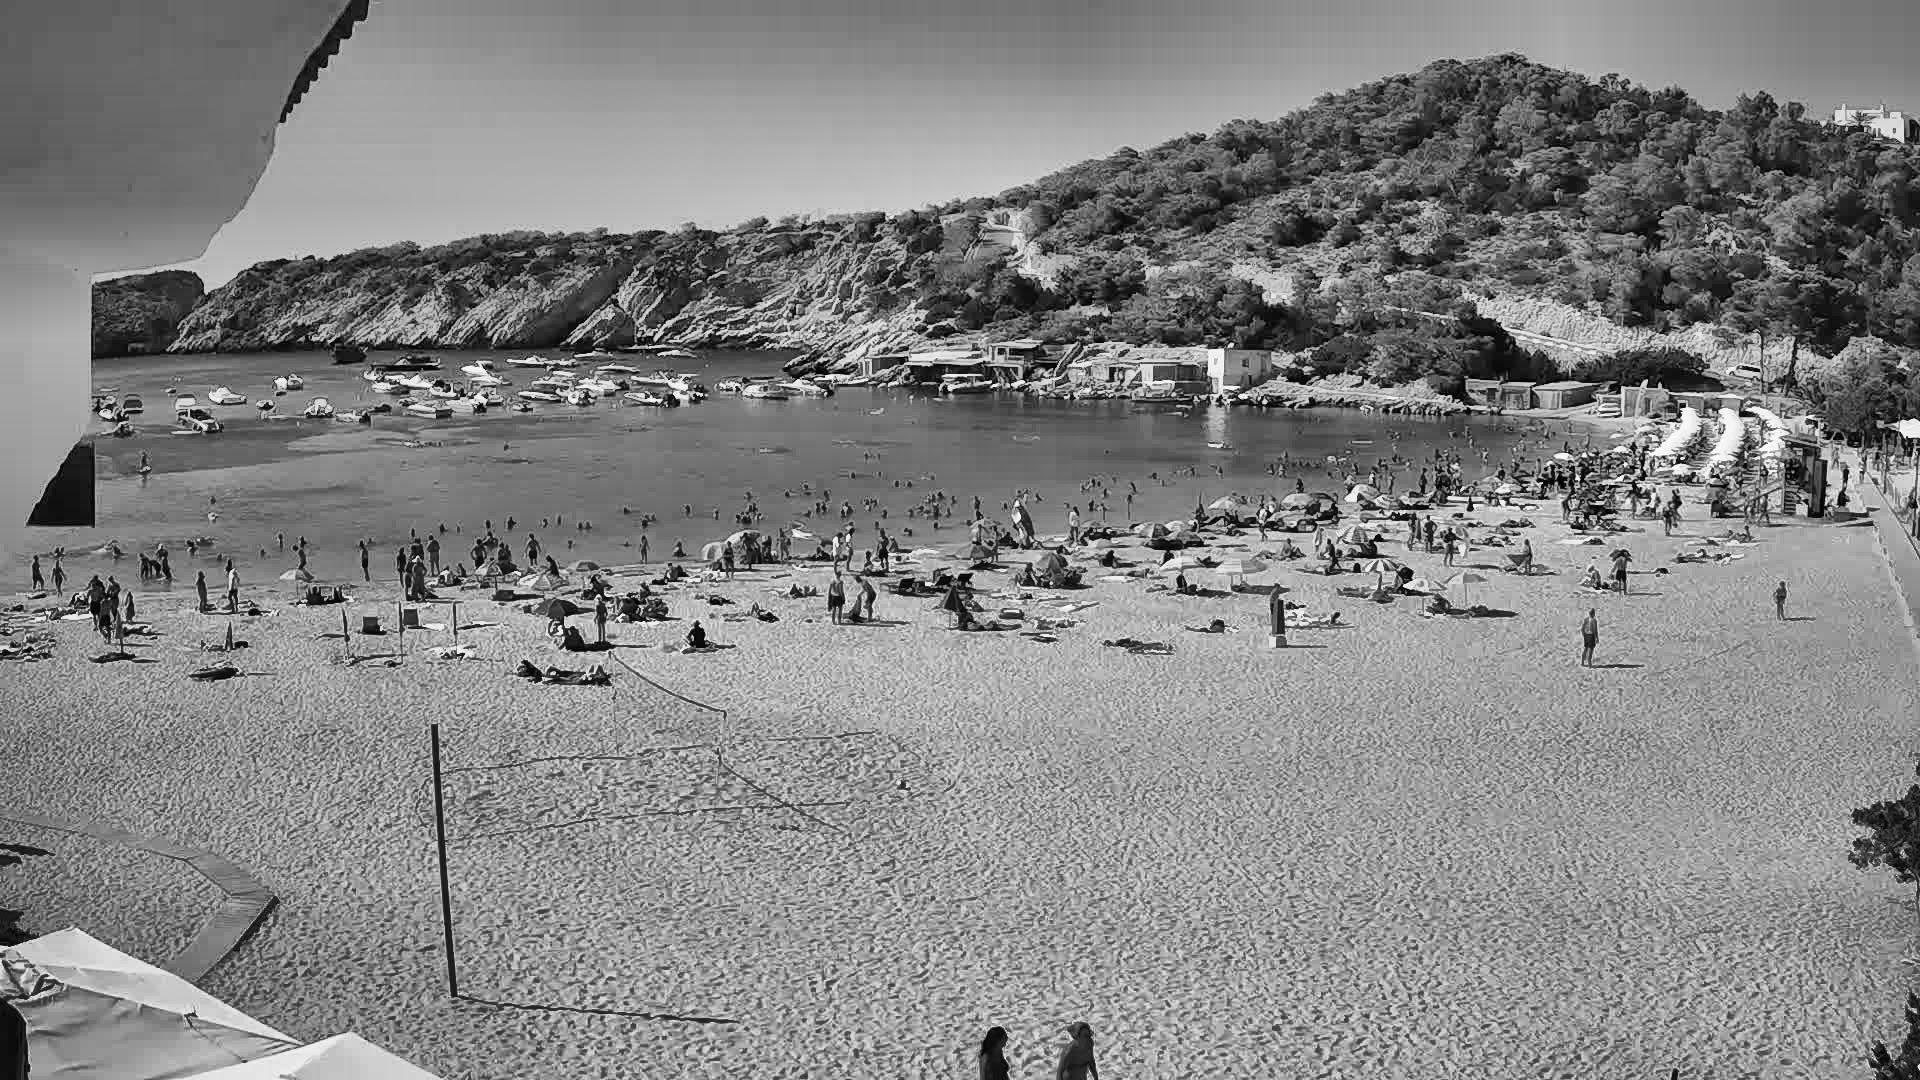
\includegraphics[width=\textwidth]{../gen/equ/1660316400.jpg} 
\end{frame}

\subsection*{Background Image}
\begin{frame}
    \frametitle{Background Image}

    \begin{figure}
        \centering
        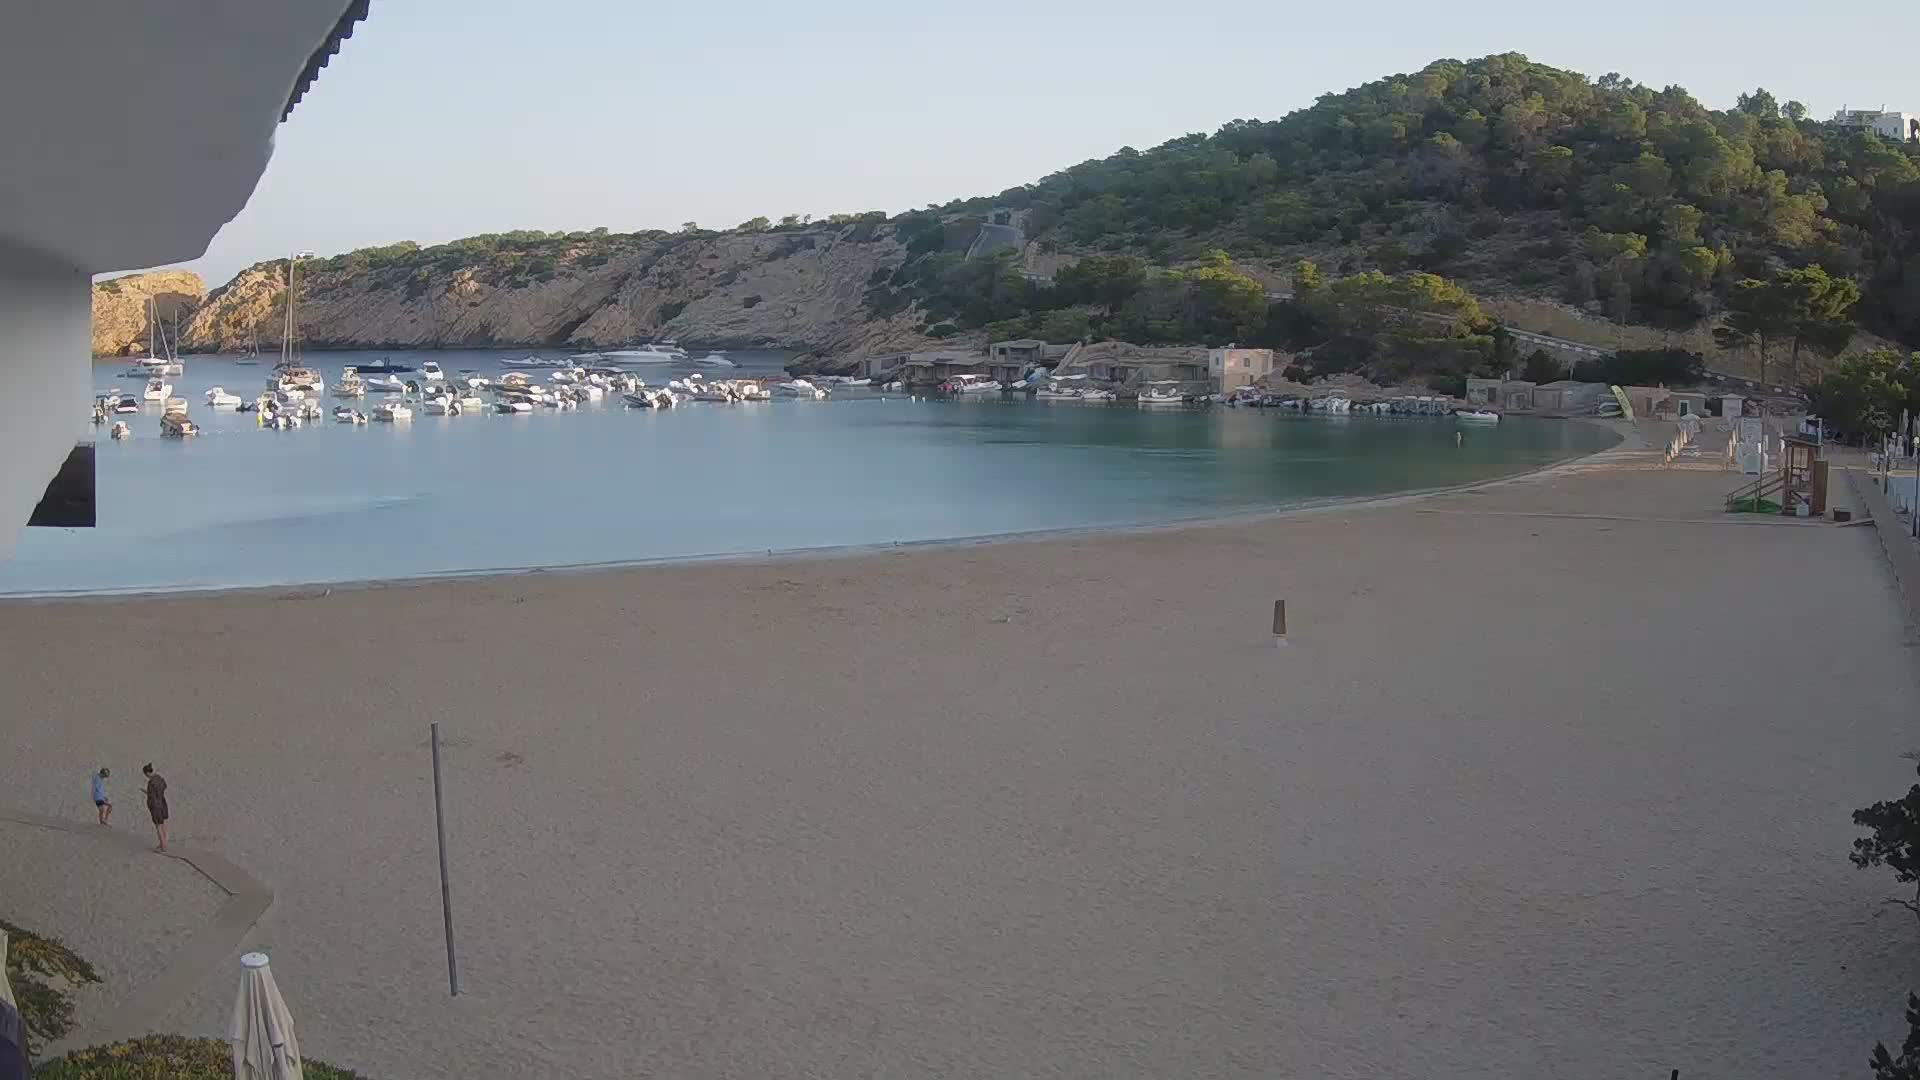
\includegraphics[width=\textwidth]{../Gelabert/1660284000.jpg}
    \end{figure}

\end{frame}

\begin{frame}
    \frametitle{Average image \ding{55}}

    \begin{figure}
        \centering
        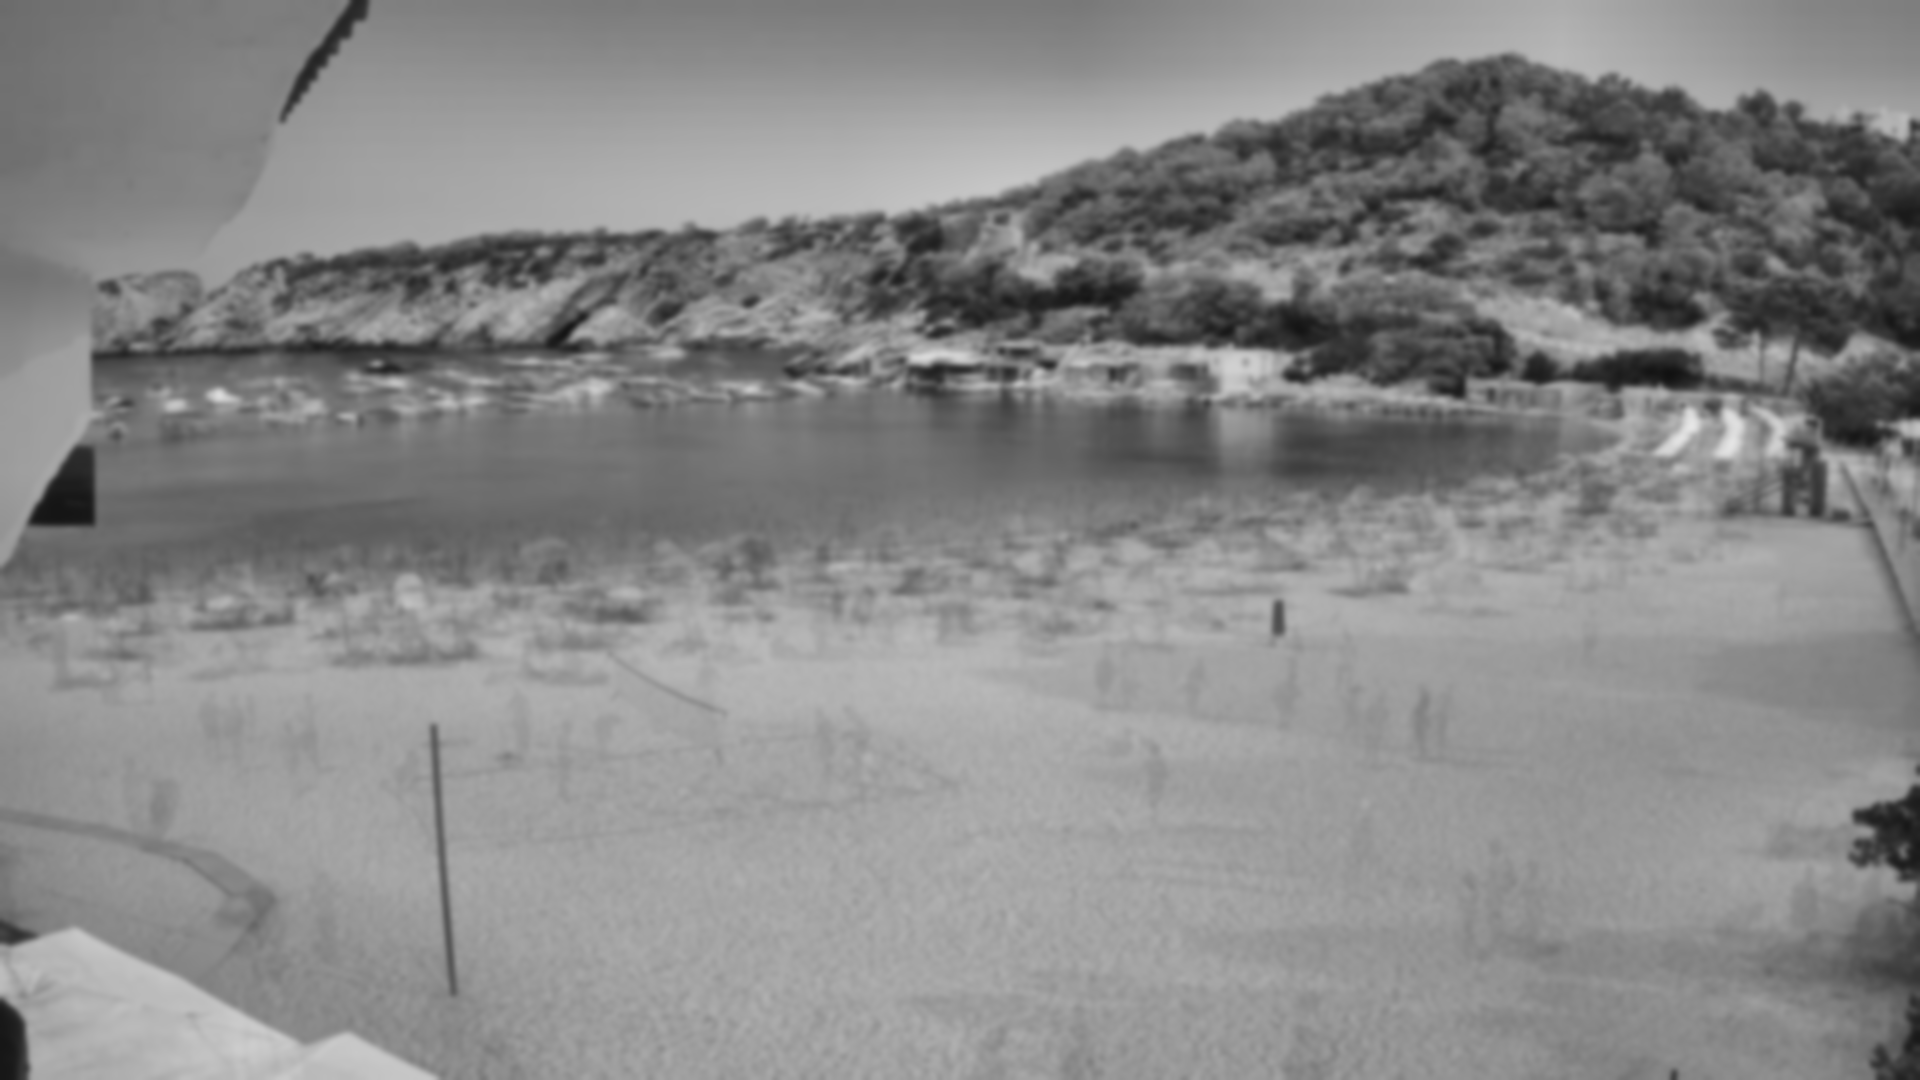
\includegraphics[width=\textwidth]{../gen/avg.png}
    \end{figure}
    
\end{frame}

\subsection*{Gaussian Blur}
\begin{frame}
    \frametitle{Gaussian Blur}
    \begin{figure}
        \centering
        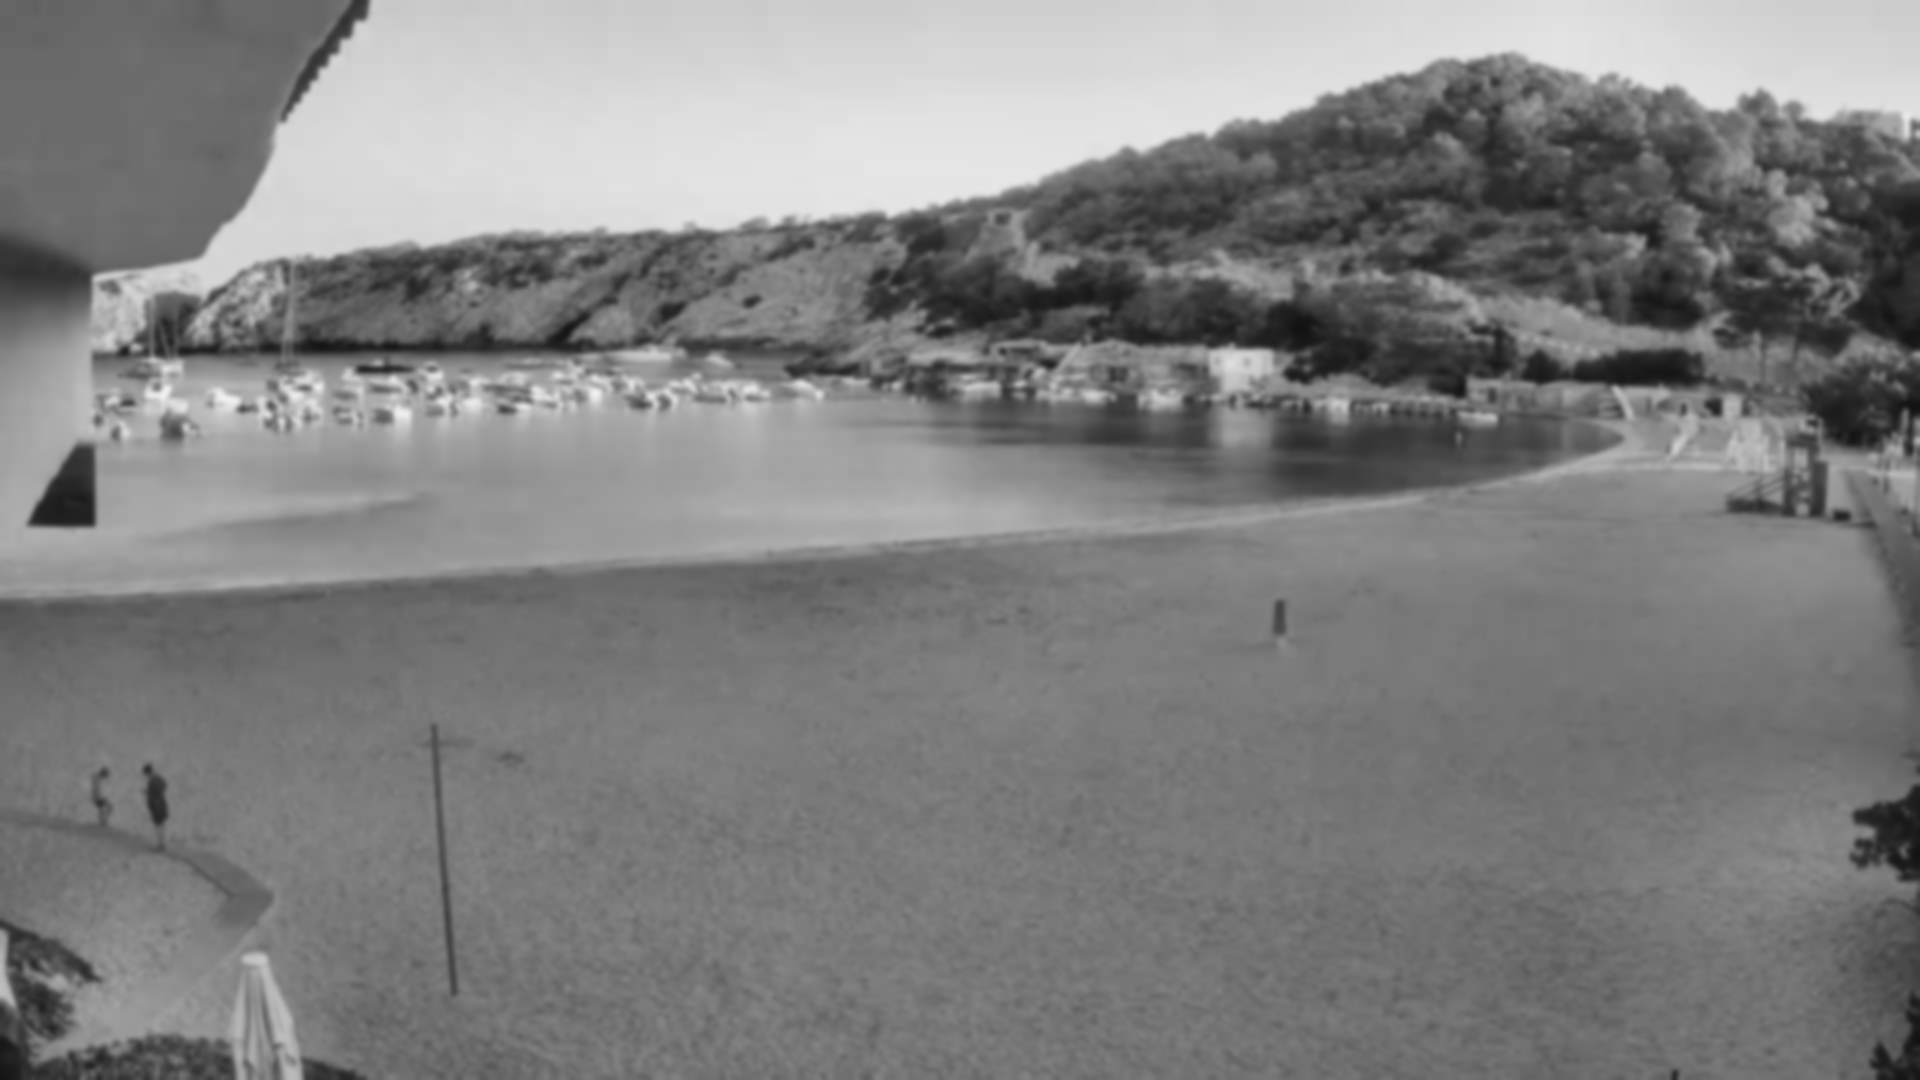
\includegraphics[width=\textwidth]{../gen/blur.png}
    \end{figure}

\end{frame}

\subsection*{Substraction}
\begin{frame}
    \frametitle{Substraction}
    \begin{figure}
        \centering
        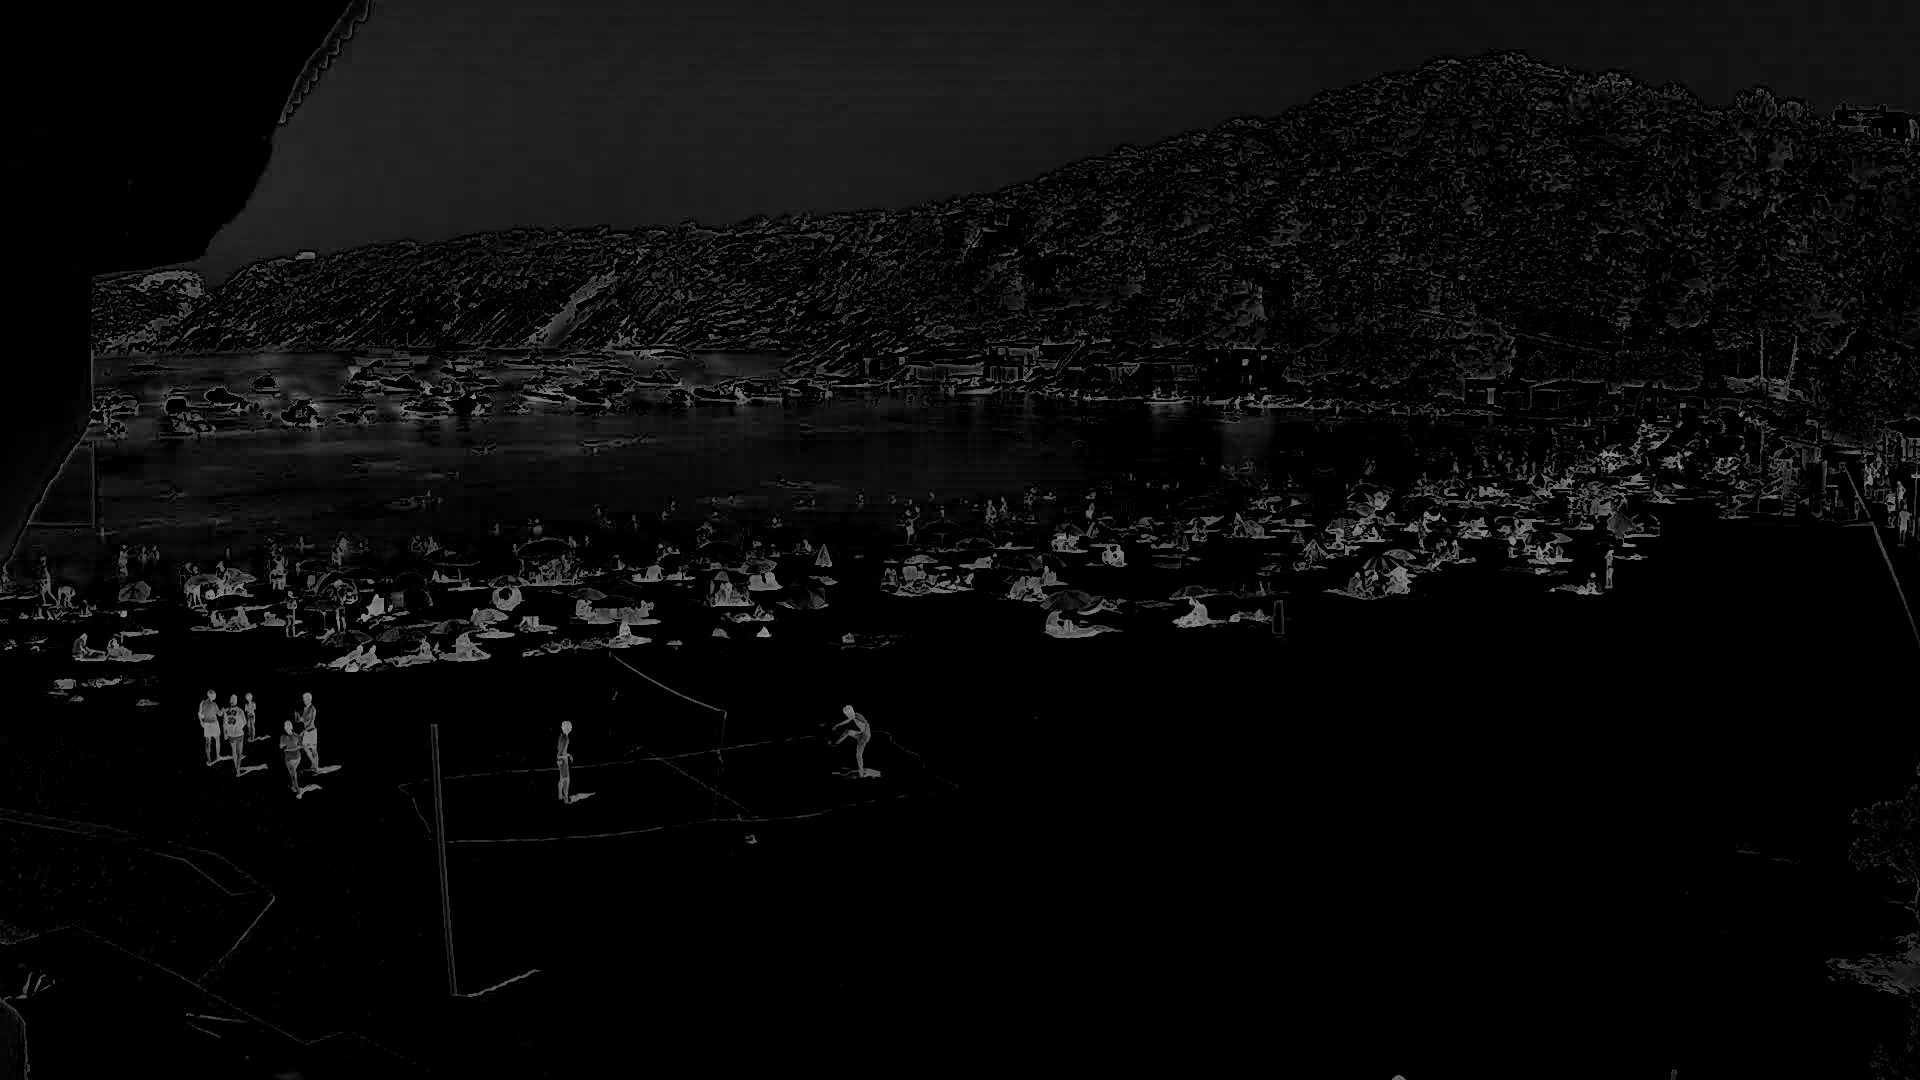
\includegraphics[width=\textwidth]{../gen/sub/1660305600.jpg}
    \end{figure}
\end{frame}

\section{Binarization}
\begin{frame}
    \frametitle{Binarization}
    \begin{figure}
        \centering
        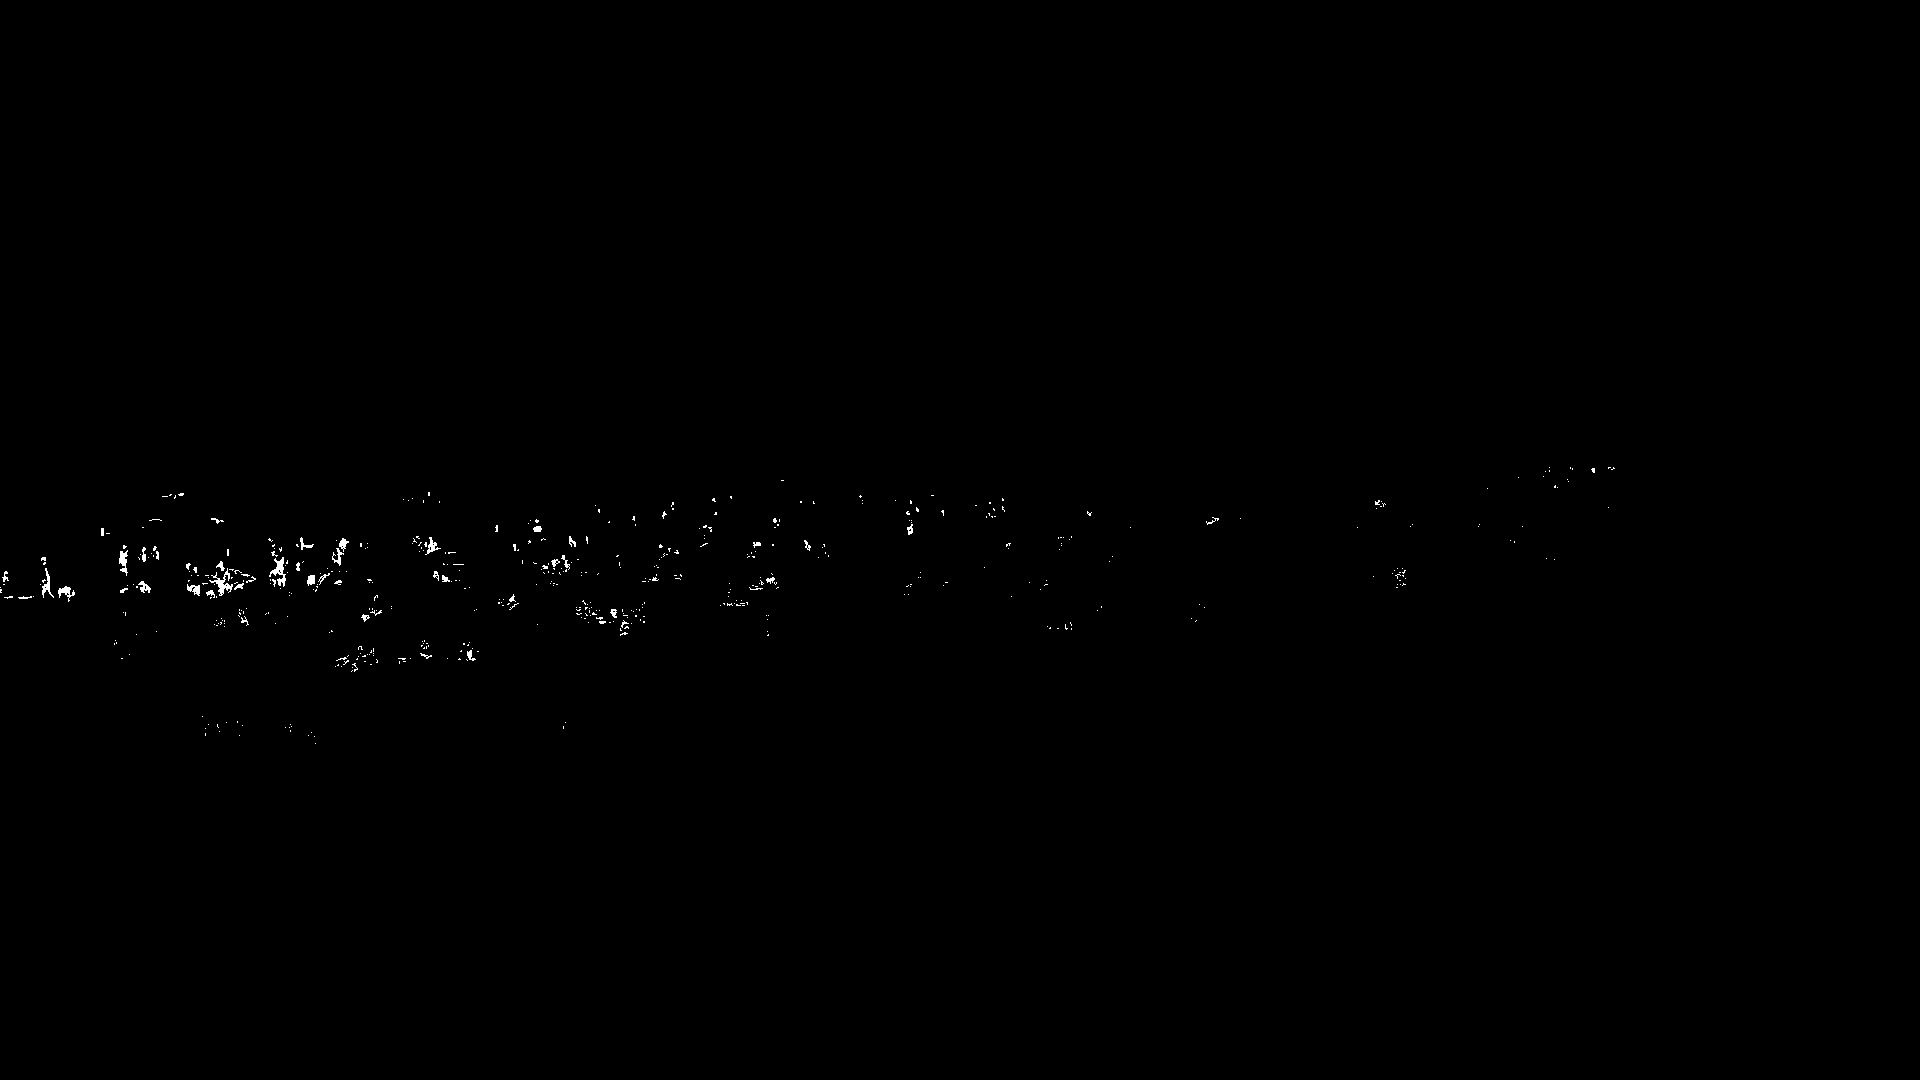
\includegraphics[width=\textwidth]{../gen/bin/1660305600.jpg}
    \end{figure}
   
        cv2.threshold(substracted, 100, 255, cv2.THRESH\_BINARY)
\end{frame}

\begin{frame}
    \frametitle{OTSU \ding{55}}
    \begin{figure}
        \centering
        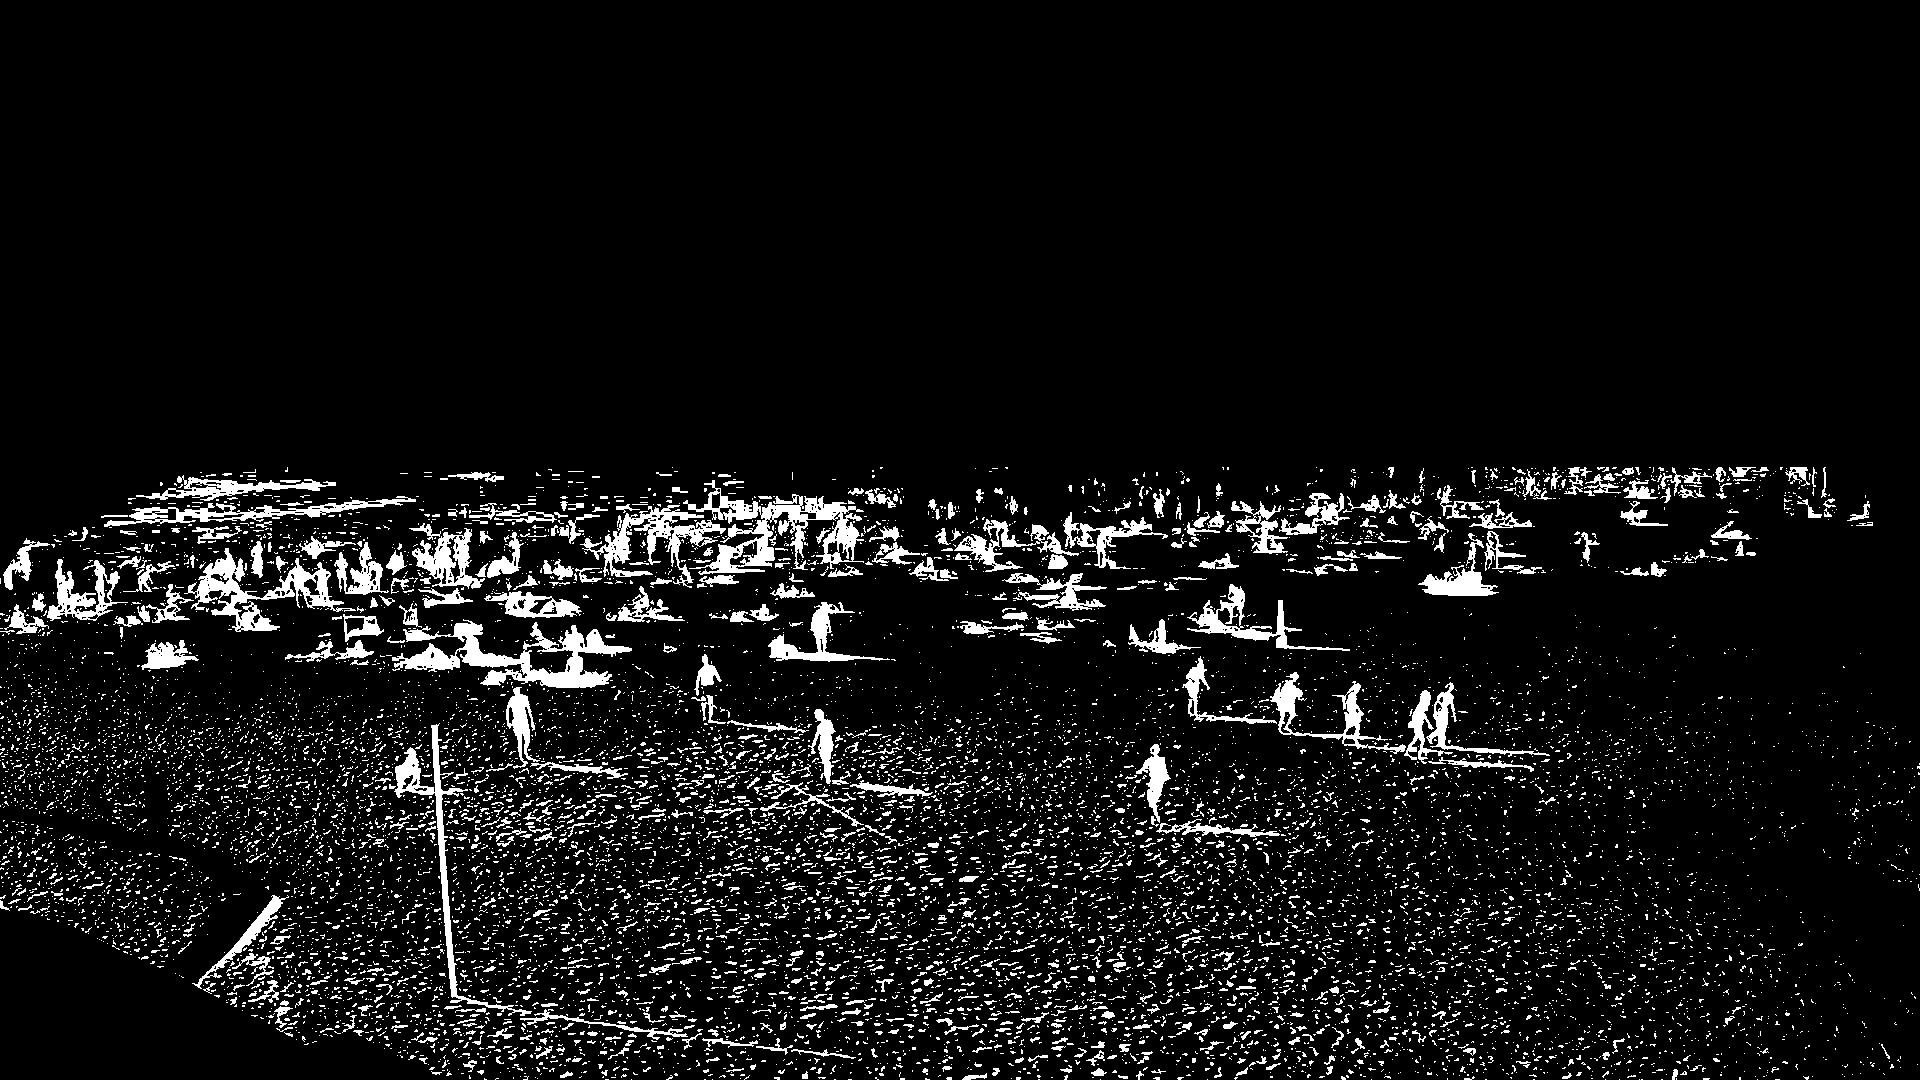
\includegraphics[width=\textwidth]{../Documentation/img/OTSU_sub_arena.jpg}
    \end{figure}
\end{frame}

\subsection*{Masking}
\begin{frame}
    \frametitle{Masking}
    \begin{figure}
        \centering
        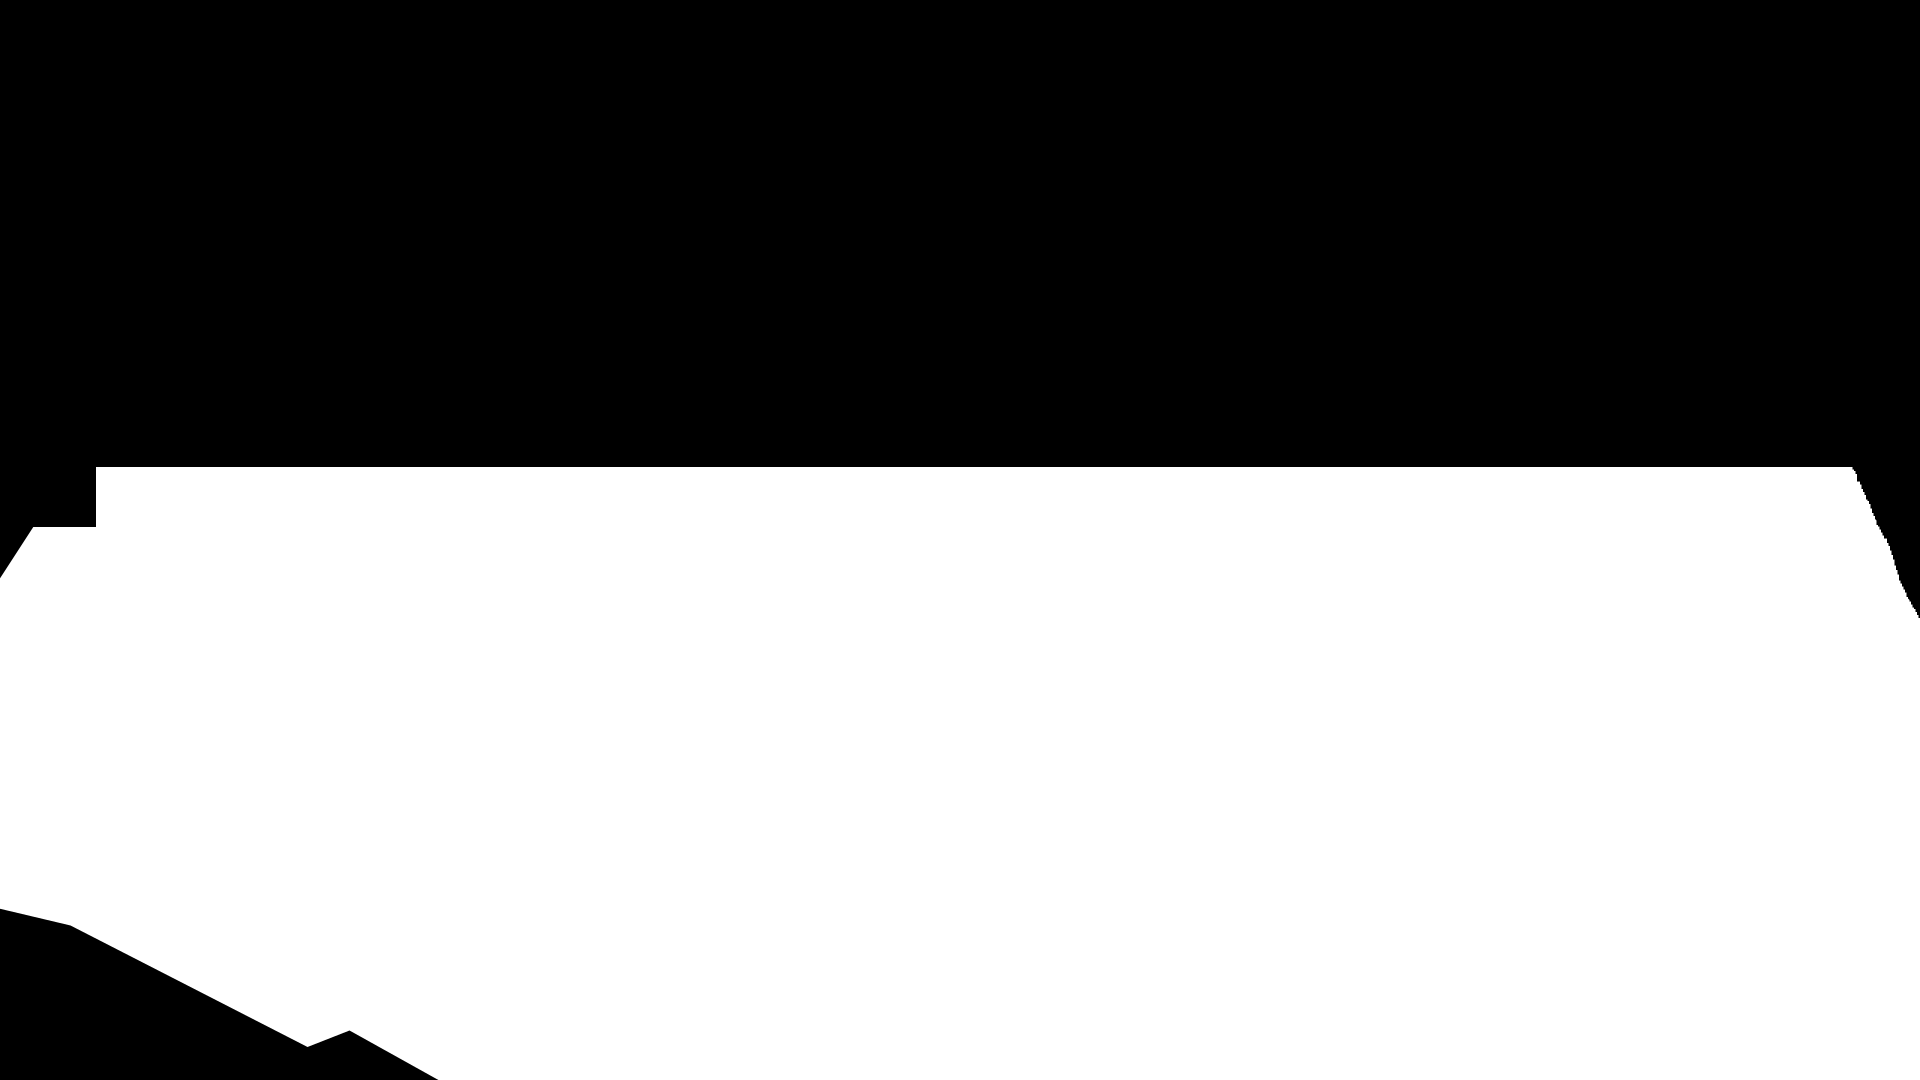
\includegraphics[width=\textwidth]{../mask.png}
    \end{figure}
\end{frame}

\section{Dilation}
\begin{frame}
    \frametitle{Dilation}

    \begin{figure}
        \centering
        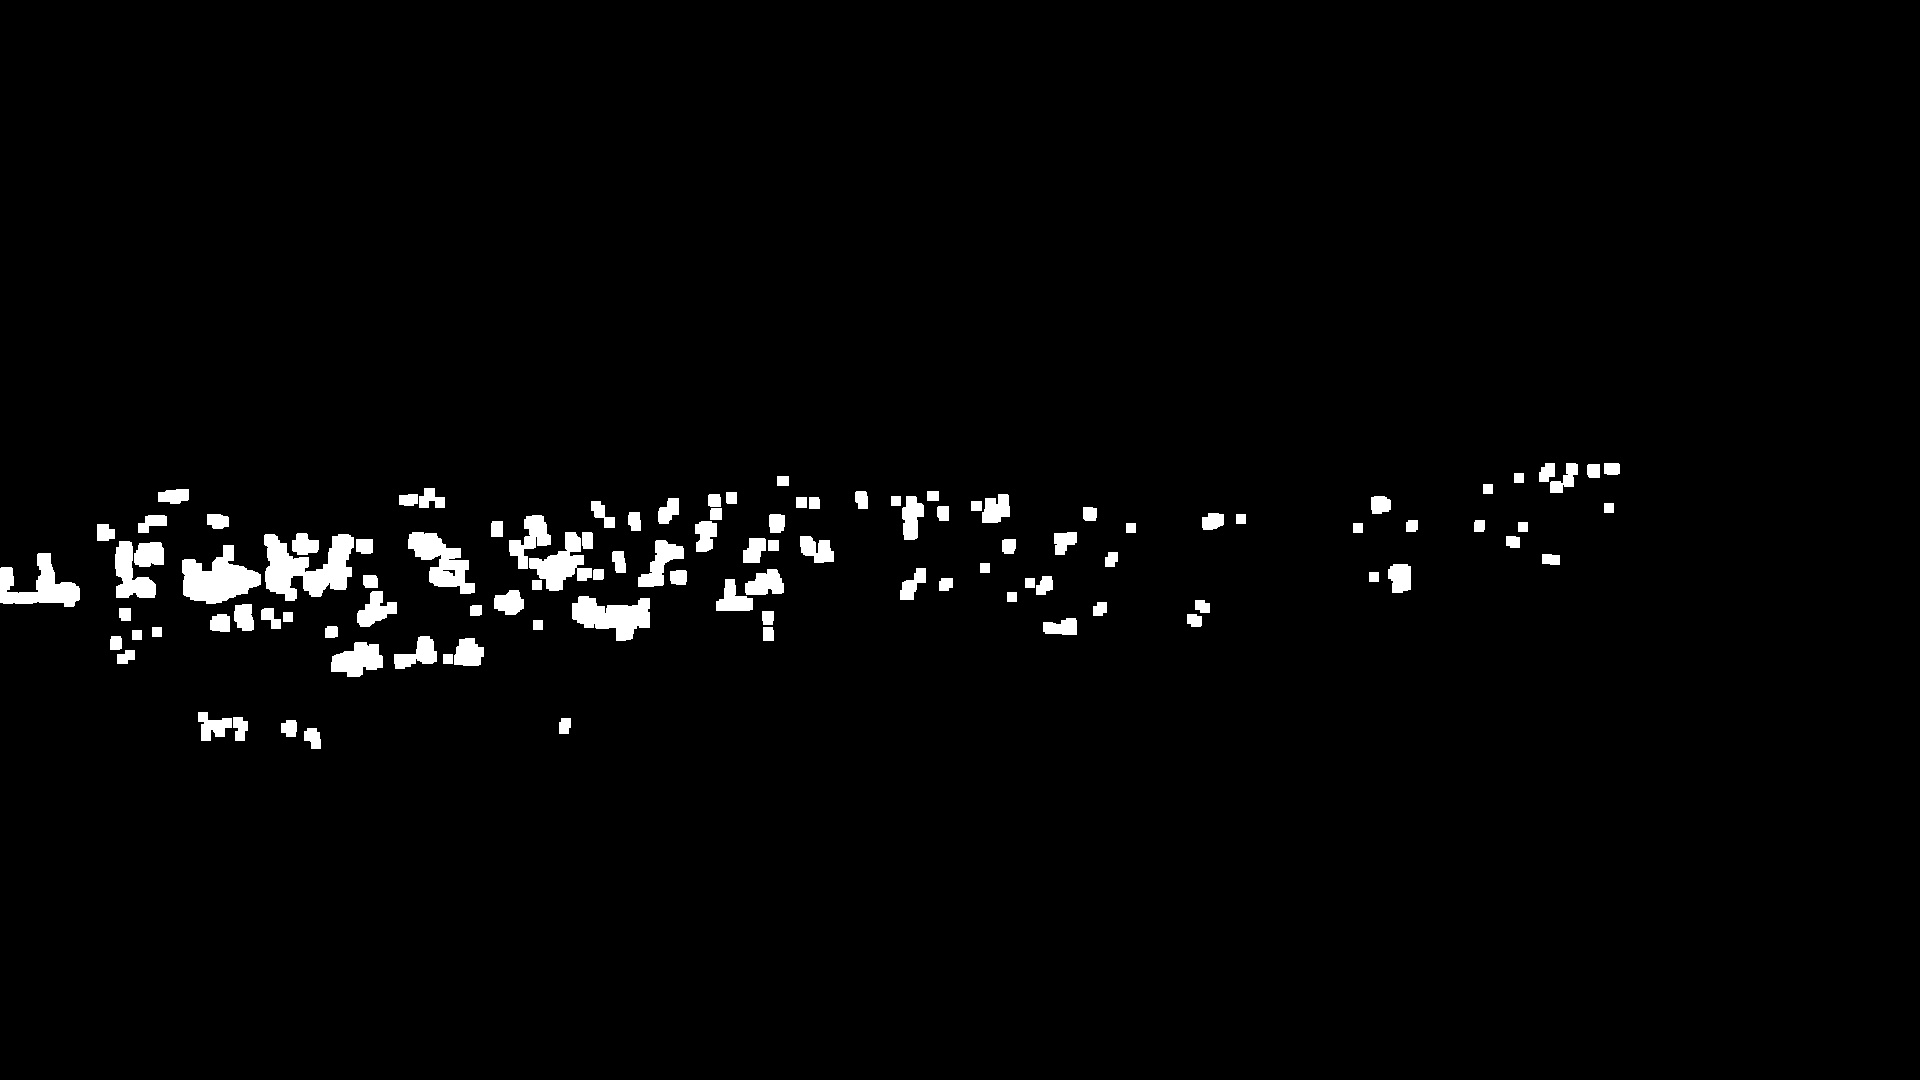
\includegraphics[width=\textwidth]{../gen/dil/1660305600.jpg}
    \end{figure}

    
\end{frame}

\section{Find contours}
\begin{frame}
    \frametitle{Output}
    \begin{figure}
        \centering
        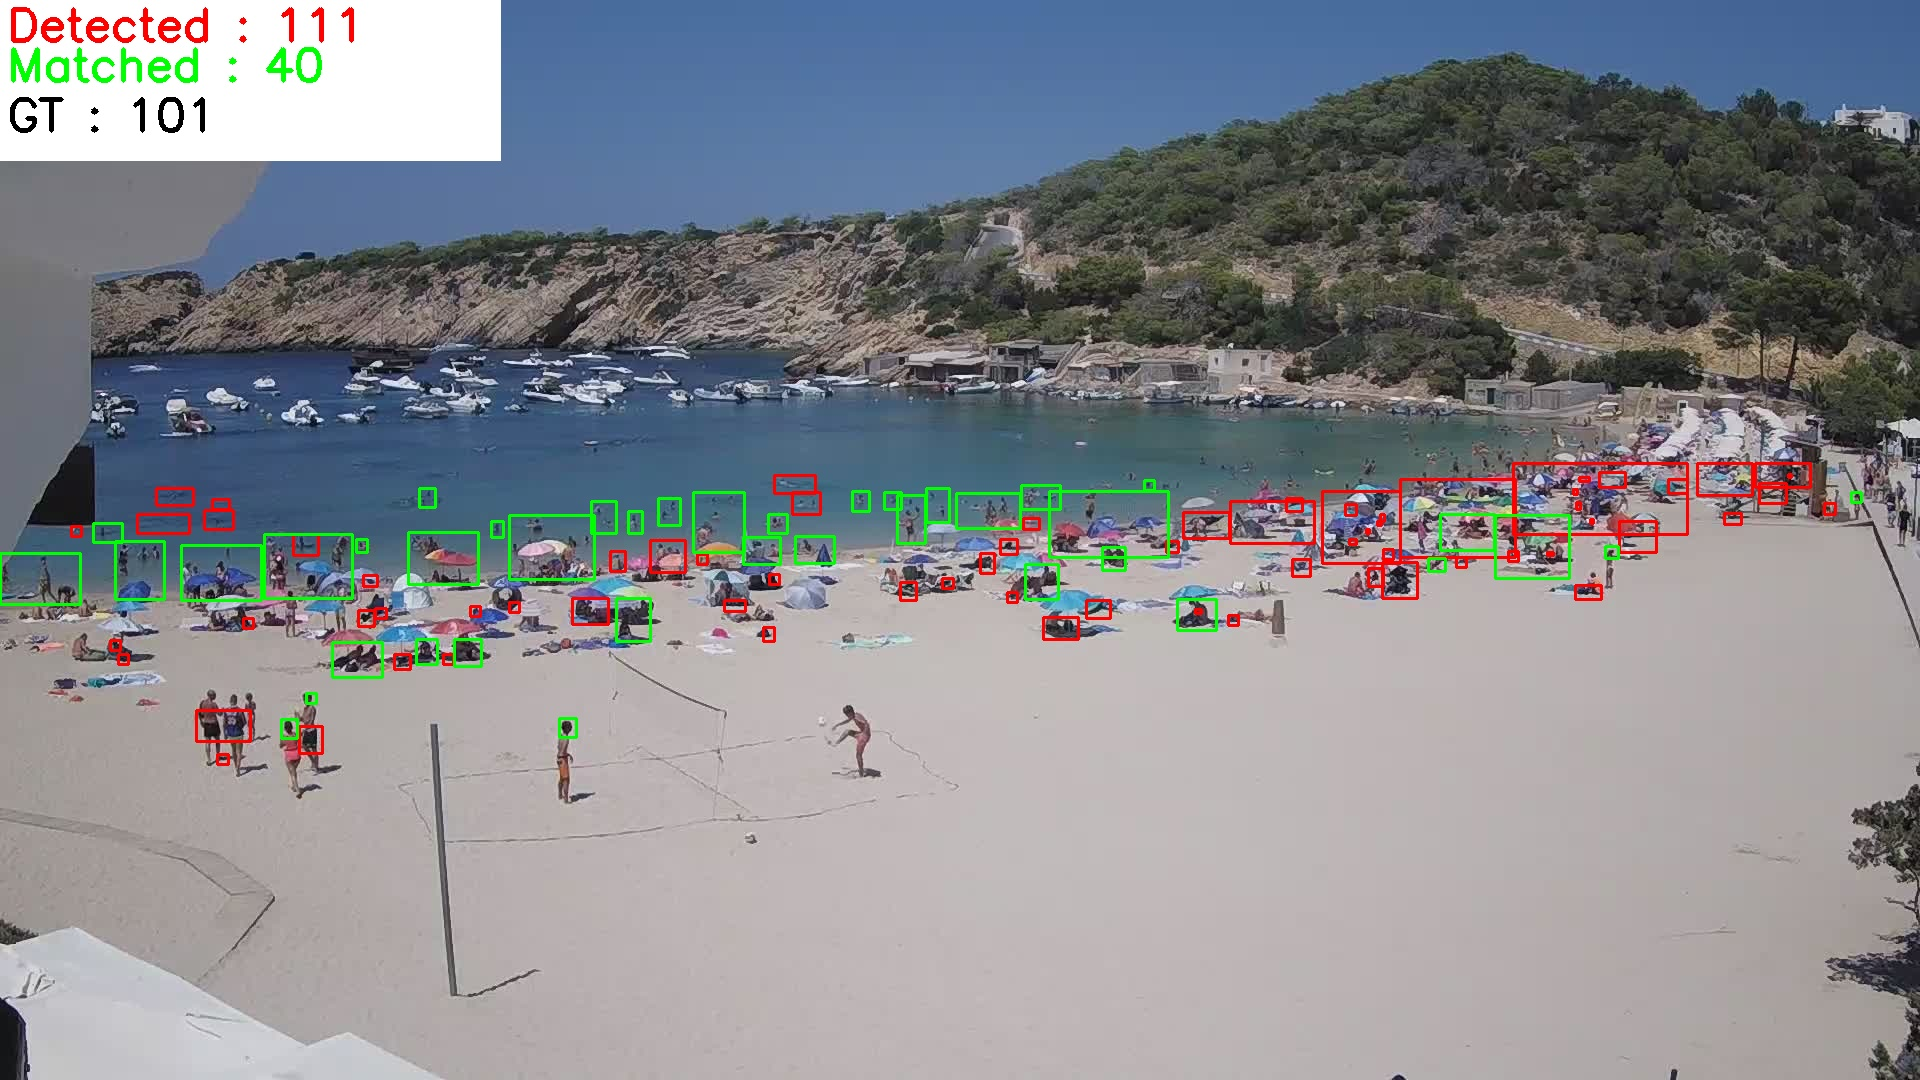
\includegraphics[width=\textwidth]{../gen/det/1660305600.jpg}
    \end{figure}
\end{frame}


\section{Results}

\begin{frame}
    \frametitle{Evaluation}
    \begin{itemize}
        
    \item Only detections containing labels will be considered \textbf{TP}.
    \item If detection contains more than one person it will count as only one detection.
    \item Massive or tiny regions will be discarded.
    \item Some labels of the ground truth could be double checked.
\end{itemize}
\end{frame}

\begin{frame}
    \frametitle{Results}
    \resizebox{\textwidth}{!}{%
    %\begin{table}
        %\centering
        %\caption[Performance metrics Basic]{Performance metrics using the propossed algorithm (withouth using the empty image)}\label{table:metrics}
    \csvautobooktabular{../metrics.csv}
    %\end{table}
    }
    %\newline \newline \newline
    %MSE = \input{../MSE.txt}
\end{frame}

\begin{frame}
    \frametitle{Results}
    \resizebox{\textwidth}{!}{%

    \csvautobooktabular{../metrics_2.csv}

    }

\end{frame}

\section{Outputs}
\foreach \name in \List {%
  \beamerfigure{\name}%
}%

\section{Conclusions}
\begin{frame}
    \frametitle{Conclusions}
    \begin{itemize}
        \item Not seeking perfect detection.
        \item Brusque changes confuse our algorithm (i.e. cast shadows).
        \item Working in color could be not ideal.
        \item The results are really fragile.
    \end{itemize}
\end{frame}


\begin{frame}
    \frametitle{Thank you!}
    
        Any Questions?
    
\end{frame}

\end{document}